% !TeX program = pdflatex

%\documentclass[handout,aspectratio=169,table,x11names,dvipsnames]{beamer}
\documentclass[aspectratio=169,table,x11names,dvipsnames]{beamer}
\usepackage{zref-abspage}

\setbeamertemplate{navigation symbols}{}


% basic includes
\usepackage[utf8]{inputenc}
\usepackage{zref-abspage}
\usepackage{graphicx}
\usepackage{amssymb}
\usepackage{animate}
\usepackage{appendixnumberbeamer}
\usepackage[USenglish]{babel}
\usepackage{caption}
\captionsetup[figure]{labelformat=empty}
\usepackage{etoolbox}

% \usepackage[utf8]{inputenc}
\usepackage{interval}
\usepackage{lmodern}
\usepackage{marvosym}
\usepackage{multicol}
\usepackage{setspace}
\usepackage{tabularx}
\usepackage{transparent}
\usepackage{varwidth}
\usepackage{xcolor}
\usepackage{xspace}
\usepackage{xkeyval}



%% BEAMER theme specifics
\usetheme{default}
\setbeamertemplate{navigation symbols}{}

% patch vertical padding between toc entries
\makeatletter
\patchcmd{\beamer@sectionintoc}{\vskip1.5em}{\vskip0.3em}{}{}
\makeatother

% custom footline -> necessary or [plain] won't work
\setbeamertemplate{sidebar right}{}
\setbeamertemplate{footline}{%
\hfill\hspace{1cm}\textcolor{structure.fg}{\insertframenumber{}/\inserttotalframenumber}\hspace{.3em}\vspace{.3em}}

% add background images to section toc slides
\AtBeginSection[]{
    {

      \IfFileExists{%
        % CONDITION
        figures/backgrounds/\thesection.png}{%
        % TRUE
        \usebackgroundtemplate{%
          \vbox to \paperheight{\vfil\hbox to \paperwidth{\hfil\transparent{0.15}\includegraphics[width=\paperwidth, height=\paperheight, keepaspectratio]{figures/backgrounds/\thesection.png}\hfil}\vfil}
        }
      }{%
        % FALSE
      }
      \IfFileExists{%
        % CONDITION
        figures/backgrounds/\thesection.pdf}{%
        % TRUE
        \usebackgroundtemplate{%
          \vbox to \paperheight{\vfil\hbox to \paperwidth{\hfil\transparent{0.15}\includegraphics[width=\paperwidth, height=\paperheight, keepaspectratio]{figures/backgrounds/\thesection.pdf}\hfil}\vfil}
        }
      }{%
        % FALSE
      }

  \begin{frame}
    \frametitle{Bonus Material: \insertsection }
    \begin{multicols}{2}
        \setbeamertemplate{section in toc}{\raggedright \leftskip=1.6em \parindent=-1.6em \textcolor{structure.fg}{$\blacktriangleright$}\hspace{.5 em}~\inserttocsection\\}
        \setbeamertemplate{subsection in toc}{\raggedright \leftskip=1.9em \parindent=-1.9em \hspace{1.3 em}--\hspace{.2 em}~\inserttocsubsection\\}


        \setbeamerfont{section in toc}{series=\bf}
        \setbeamerfont{subsection in toc}{series=\bf}

        \setbeamerfont{section in toc shaded}{series=\normalfont}
        \setbeamerfont{subsection in toc shaded}{series=\normalfont}
        \setbeamertemplate{section in toc shaded}[default][65]
        \setbeamertemplate{subsection in toc shaded}[default][65]
        \tableofcontents[currentsection,subsectionstyle=show/show/shaded]
    \end{multicols}
  \end{frame}
  }
}

% change the Appendix name to Bonus Material (mainly in PDF viewer navigation bar)
\usepackage{appendix}
\addto{\captionsUSenglish}{\renewcommand*{\appendixname}{Bonus Material}}
\addto{\captionsUSenglish}{\renewcommand*{\appendixtocname}{Bonus Material}}
\addto{\captionsUSenglish}{\renewcommand*{\appendixpagename}{Bonus Material}}

% remove hyperref warning
\usepackage{hyperref}
\pdfstringdefDisableCommands{%
  \def\\{}%
  \def\texttt#1{<#1>}%
}

% per default use inline TODOs and remove warning
\usepackage{todonotes}
\presetkeys{todonotes}{inline}{}
\setlength {\marginparwidth }{2cm}

% add new (non-SI) units
\usepackage{siunitx}
\sisetup{
	per-mode=fraction,
	fraction-function=\tfrac
}
\DeclareSIUnit{\month}{m} 	 % Month
\DeclareSIUnit{\year}{y} 	 % Year
\DeclareSIUnit{\radian}{rad} % Radian
\DeclareSIUnit{\au}{AU} 	 % Astronomical Unit
\DeclareSIUnit{\jd}{JD} 	 % Julian Day


% use special tikz libraries and overwrite the default arrow head
\tracinglostchars=2
\usepackage{tikz}
\usetikzlibrary{
   shadings,
   shadows,
   positioning,
   arrows.meta,
   decorations.pathreplacing,
}
\tikzset{
	% draw a simple CPU
    >={Latex[length=2mm, width=1.25mm]},
    pics/cpu/.style n args={1}{%
        code={
\draw (0, 0) rectangle (2, 2);
\node at (1, .25) {CPU #1};
\draw (0.15, 1.35) rectangle (0.85, 1.85);
\draw[fill=red] (0.225, 1.475) rectangle (0.45, 1.725);
\draw[fill=BurntOrange] (0.55, 1.475) rectangle (0.775, 1.725);

\draw (1.15, 1.35) rectangle (1.85, 1.85);
\draw[fill=red] (1.225, 1.475) rectangle (1.45, 1.725);
\draw[fill=BurntOrange] (1.55, 1.475) rectangle (1.775, 1.725);

\draw (0.15, 0.65) rectangle (0.85, 1.15);
\draw[fill=red] (0.225, 0.775) rectangle (0.45, 1.025);
\draw[fill=BurntOrange] (0.55, 0.775) rectangle (0.775, 1.025);

\draw (1.15, 0.65) rectangle (1.85, 1.15);
\draw[fill=red] (1.225, 0.775) rectangle (1.45, 1.025);
\draw[fill=BurntOrange] (1.55, 0.775) rectangle (1.775, 1.025);
        }%
    }%
}

% overwrite default minted background
\usepackage{minted}
\setminted{
    bgcolor=lightgray!30
}

% add new math commands
\usepackage{mathtools}
\DeclarePairedDelimiter\abs{\lvert}{\rvert}
\DeclarePairedDelimiter\norm{\lVert}{\rVert}
\makeatletter
\let\oldabs\abs
\def\abs{\@ifstar{\oldabs}{\oldabs*}}
%
\let\oldnorm\norm
\def\norm{\@ifstar{\oldnorm}{\oldnorm*}}
\makeatother

% add algorithm environment without the need for a caption
\usepackage{algorithm,algpseudocode}
\newenvironment{algorithmcl}
 {\par\addvspace{\topsep}
  \centering
  \begin{minipage}{\linewidth}
  \hrule\kern2pt}
 {\par\kern2pt\hrule
  \end{minipage}
  \par\addvspace{\topsep}}

% add better arrow
\usepackage{fontawesome5}
\newcommand{\DisplayRightArrow}{\faIcon{arrow-right}\xspace}
% add arrow that is correctly displayed even with multiple lines
\newcommand{\itFollows}[1]{%
	\begin{tabularx}{\textwidth}{rX}
		\DisplayRightArrow & #1
	\end{tabularx}
}



% set fontsize to a specific pt value
\newcommand{\setfontsize}[1]{\fontsize{#1pt}{1.2\dimexpr#1pt\relax}\selectfont}

% better automatic quotes
\usepackage{csquotes}


% vill slide to the bottom
\newcommand{\btVFill}{\vskip0pt plus 1filll}
% mark links with symbol
\newcommand{\link}[2]{\href{#1}{#2\,\textsuperscript{\color{gray}\tiny\faIcon{external-link-alt}}}}
\def\dateKickoffPhaseOne{25.10.2023}
\def\dateDeadlinePhaseZero{02.11.2023}
\def\dateKickoffPhaseTwo{27.11.2023}
\def\dateDeadlinePhaseOne{04.12.2023}
\def\dateDeadlinePhaseTwo{29.01.2024}
\def\dateFinal{TBA}

\def\urlIliasCourse{https://ilias3.uni-stuttgart.de/goto_Uni_Stuttgart_crs_3426920.html}
\def\urlIliasForumGeneral{https://ilias3.uni-stuttgart.de/goto_Uni_Stuttgart_frm_3451473.html}
\def\urlIliasForumGroups{https://ilias3.uni-stuttgart.de/goto_Uni_Stuttgart_frm_3451472.html}
\def\urlIliasData{https://ilias3.uni-stuttgart.de/goto_Uni_Stuttgart_fold_3451475.html}
\def\urlIliasSubmissionPhaseZero{https://ilias3.uni-stuttgart.de/goto_Uni_Stuttgart_exc_3451474.html}
\def\urlIliasSubmissionPhaseOne{https://ilias3.uni-stuttgart.de/goto_Uni_Stuttgart_exc_3451474.html}
\def\urlIliasSubmissionPhaseTwo{https://ilias3.uni-stuttgart.de/goto_Uni_Stuttgart_exc_3451474.html}
\def\urlIliasSubmissionFinal{https://ilias3.uni-stuttgart.de/goto_Uni_Stuttgart_exc_3451474.html}
\def\urlIliasLatexTemplate{https://ilias3.uni-stuttgart.de/goto_Uni_Stuttgart_exc_3451474.html}
\def\semester{Summerterm 2024}

\def\supervisorAc{\texttt{ac127328} und \texttt{ac127336}}
\def\urlNextcloud{https://ipvs.informatik.uni-stuttgart.de/cloud/s/4HbjLCQmfbenpWq}
\def\passwordNextcloud{TODO}

\usetheme[
	totalframenumber,
	sectionslide,
	titleimage=figures/title_image.png,
]{uniS}

% information for the title page
\title{Lab Course:\\ Solar System \\Simulation}
\cclicense{by-nc-sa}

\institute[logo=.logos/ipvslogo_rund_blau_dunkel.pdf, url=https://www.ipvs.uni-stuttgart.de/]{Institute for Parallel and Distributed Systems}{IPVS}

\department[logo=.logos/logo_scientific_comp.pdf, url=https://www.ipvs.uni-stuttgart.de/departments/sc/]{Scientific Computing}{SC}

\author[Van Craen, Breyer, Prof. Pflüger]{Alexander Van Craen,\\Marcel Breyer,\\Prof. Dr. Dirk Pflüger}
\date{\semester}

\begin{document}



\titleslide


%%%%%%%%%%%%%%%%%%%%%%%%%%%%%%%%%%%%%%%%%%%%%%%%%%%%%%%%%%%%%%%%%%%%
\begin{frame}[c]{Who are we?}
    \setfontsize{9}
    \begin{columns}[c]
    	\begin{column}{0.3\textwidth}
			\centering
			\begin{tikzpicture}
				\node[circle, minimum size=2cm, path picture={\node at (path picture bounding box.center){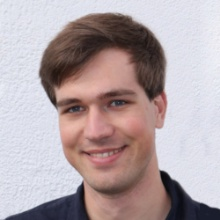
\includegraphics[height=2cm]{figures/speaker/AlexanderVanCraen}};}] {};
			\end{tikzpicture} \\
			\textbf{Alexander Van Craen} \\[.4em]
			\href{mailto:Alexander.Van-Craen@ipvs.uni-stuttgart.de}{Alexander.Van-Craen@ipvs.uni-stuttgart.de}
		\end{column}
    	\begin{column}{0.3\textwidth}
    		\centering
			\begin{tikzpicture}
				\node[circle,minimum size=2cm, path picture={\node at (path picture bounding box.center){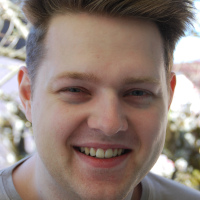
\includegraphics[height=2cm]{figures/speaker/MarcelBreyer}};}] {};
			\end{tikzpicture} \\
			\textbf{Marcel Breyer} \\[.4em]
			\href{mailto:Marcel.Breyer@ipvs.uni-stuttgart.de}{Marcel.Breyer@ipvs.uni-stuttgart.de}
    	\end{column}
    	\begin{column}{0.3\textwidth}
    		\centering
			\begin{tikzpicture}
				\node[circle,minimum size=2cm, path picture={\node at (path picture bounding box.center){
\includegraphics[height=2cm]{figures/speaker/LinusBantel}};}] {};
			\end{tikzpicture} \\
			\textbf{Linus Bantel} \\[.4em]
			\href{mailto:Linus.Bantel@ipvs.uni-stuttgart.de}{Linus.Bantel@ipvs.uni-stuttgart.de}
    	\end{column}
    \end{columns}
	\vspace*{1.5em}
	\begin{columns}
		\begin{column}{0.3\textwidth}
			\centering
			\begin{tikzpicture}
				\node[circle,minimum size=2cm, path picture={\node at (path picture bounding box.center){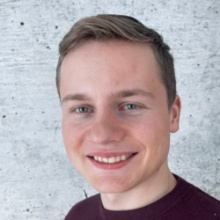
\includegraphics[height=2cm]{figures/speaker/AlexanderStrack}};}] {};
			\end{tikzpicture} \\
			\textbf{Alexander Strack} \\[.4em]
			\href{mailto:Alexander.Strack@ipvs.uni-stuttgart.de}{Alexander.Strack@ipvs.uni-stuttgart.de}
		\end{column}
		\begin{column}{0.3\textwidth}
			\centering
			\begin{tikzpicture}
				\node[circle,minimum size=2cm, path picture={\node at (path picture bounding box.center){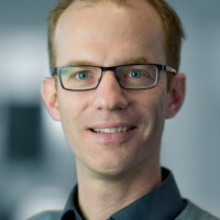
\includegraphics[height=2cm]{figures/speaker/DirkPflueger}};}] {};
			\end{tikzpicture} \\
			\textbf{Prof. Dr. Dirk Pflüger} \\[.4em]
			\href{mailto:Dirk.Pflueger@ipvs.uni-stuttgart.de}{Dirk.Pflueger@ipvs.uni-stuttgart.de}
		\end{column}
	\end{columns}
\end{frame}
%%%%%%%%%%%%%%%%%%%%%%%%%%%%%%%%%%%%%%%%%%%%%%%%%%%%%%%%%%%%%%%%%%%%


%%% input basic slides -> most important slides
\section*{Outline}
%%%%%%%%%%%%%%%%%%%%%%%%%%%%%%%%%%%%%%%%%%%%%%%%%%%%%%%%%%%%%%%%%%%%
\begin{frame}
  \frametitle{Learning Goals}
    \begin{itemize}
        \item Implementation of a non-trivial project in a small group as well as an individual extension of it.
        \item Get a feeling for intra- and inter-node parallelization strategies and frameworks.
        \item Usage of established frameworks in the High-Performance Computing (HPC) community like \link{https://www.openmp.org/}{OpenMP} and \link{https://www.mpi-forum.org/}{MPI}.
        \item Practical application of tree data structures.
        \item Working with \texttt{C++} as one of the most widely used programming languages in HPC.
        \item Practical experiences with Git (using our \link{https://gitlab-sim.informatik.uni-stuttgart.de}{GitLab instance}; for more information about Git see \link{https://githowto.com/}{Git HowTo}) and Continuous Integration (CI) testing.
        \item Getting familiar with Linux, remote development, compute clusters, and cluster resource management software like \link{https://slurm.schedmd.com/documentation.html}{SLURM}.
        \item Usage of established programs in scientific computing (e.g., \link{https://www.paraview.org/}{ParaView} for visualization).
    \end{itemize}
\end{frame}
%%%%%%%%%%%%%%%%%%%%%%%%%%%%%%%%%%%%%%%%%%%%%%%%%%%%%%%%%%%%%%%%%%%%

%%%%%%%%%%%%%%%%%%%%%%%%%%%%%%%%%%%%%%%%%%%%%%%%%%%%%%%%%%%%%%%%%%%%
\begin{frame}
  \frametitle{Content of the Lab Course}
  \begin{itemize}
    \item Lab Course divided into multiple phases:
      \begin{description}[labelwidth=2.2cm]
        \item[Group Formation] Independent formation of groups of up to 2. \\
        (Deadline: \textbf{\dateDeadlinePhaseZero})
        \item[Phase 1] Get familiar with the n-body simulation and implement it using the tree-based Barnes-Hut algorithm on a multi-node system in the previously formed group. \\
        (Deadline: \textbf{\dateDeadlinePhaseOne})
        \item[Phase 2] Extending your previous code with an \textbf{individual} project. \\
        (Deadline: \textbf{\dateDeadlinePhaseTwo})
        \item[Final Presentation] Present your results of phase 2 in a \SI{15}{\minute} presentation. \\
        (Date: \textbf{\dateFinal})
      \end{description}\pause
      \vfill
    \item Approval of phase 1 not later than the deadline. \\
        \DisplayRightArrow Reaching phase 2 only after the successful acceptance of phase 1. \\
        \DisplayRightArrow If you finish phase 1 early and let us know, you will have more time for phase 2!
    \item In addition, there will be two small competitions at the end of phase 1 (more on that later).
  \end{itemize}
\end{frame}
%%%%%%%%%%%%%%%%%%%%%%%%%%%%%%%%%%%%%%%%%%%%%%%%%%%%%%%%%%%%%%%%%%%%

%%%%%%%%%%%%%%%%%%%%%%%%%%%%%%%%%%%%%%%%%%%%%%%%%%%%%%%%%%%%%%%%%%%%
\begin{frame}
	\frametitle{Additional Meetings}
	\begin{itemize}
		\item Every \textbf{two weeks} we will have a short mandatory meeting where every group presents their progress in a short \SI{5}{\minute} presentation.
		\item Necessary content: 
		\begin{itemize}
			\item Summary: a short summary of what you did in the last two weeks and whether to achieved your previous goals.
			\item Problems: the biggest problems you encountered. 
			\item Next Steps: the next steps you will work on in the next weeks. 
		\end{itemize}
		\item Additional remarks or questions are also welcome!
		\item A slide template can be found in \link{\urlIliasSummarySlideTemplate}{ILIAS}, but other slide templates can also be used. 
	\end{itemize}
	\vfill
	\DisplayRightArrow This is only meant as assistance for you and will not influence the final grade!
\end{frame}
%%%%%%%%%%%%%%%%%%%%%%%%%%%%%%%%%%%%%%%%%%%%%%%%%%%%%%%%%%%%%%%%%%%%

\section*{Group Formation}
%%%%%%%%%%%%%%%%%%%%%%%%%%%%%%%%%%%%%%%%%%%%%%%%%%%%%%%%%%%%%%%%%%%%
\begin{frame}[fragile]
  \frametitle{Group Formation}
  % number of possible students % group size = 0 !!!
  \begin{itemize}
      \item Independent formation of groups of up to 2 (e.g., using the \link{\urlIliasForumGroups}{ILIAS forum}).
      \item The first submission in \link{\urlIliasSubmissionPhaseZero}{ILIAS} should consist of a simple text file containing all group members and a group name used for the competition and your repository in our GitLab.
      \item Deadline: \textbf{\dateDeadlinePhaseZero}
      \item If you did not find a group until \dateDeadlinePhaseZero, contact us via email and we will assign you to a group.
      \item If you did not create an ILIAS submission and did not contact us via email, you do not count as a participant in this lab course!
  \end{itemize}
\end{frame}
%%%%%%%%%%%%%%%%%%%%%%%%%%%%%%%%%%%%%%%%%%%%%%%%%%%%%%%%%%%%%%%%%%%%

\section*{Phase 1}
%%%%%%%%%%%%%%%%%%%%%%%%%%%%%%%%%%%%%%%%%%%%%%%%%%%%%%%%%%%%%%%%%%%%
\begin{frame}
	\frametitle{Phase 1: Goal}
  \vspace*{-1em}
	\begin{center}
	    Parallel, distributed n-body simulation using the tree-based Barnes-Hut algorithm of the planets, dwarf planets, moons, and asteroids in our solar system.
	\end{center}
	\vspace*{-0.75em}
	\begin{columns}
	    \begin{column}{.45\linewidth}
	        \begin{figure}
	            \centering
	            \captionsetup{justification=centering}
	            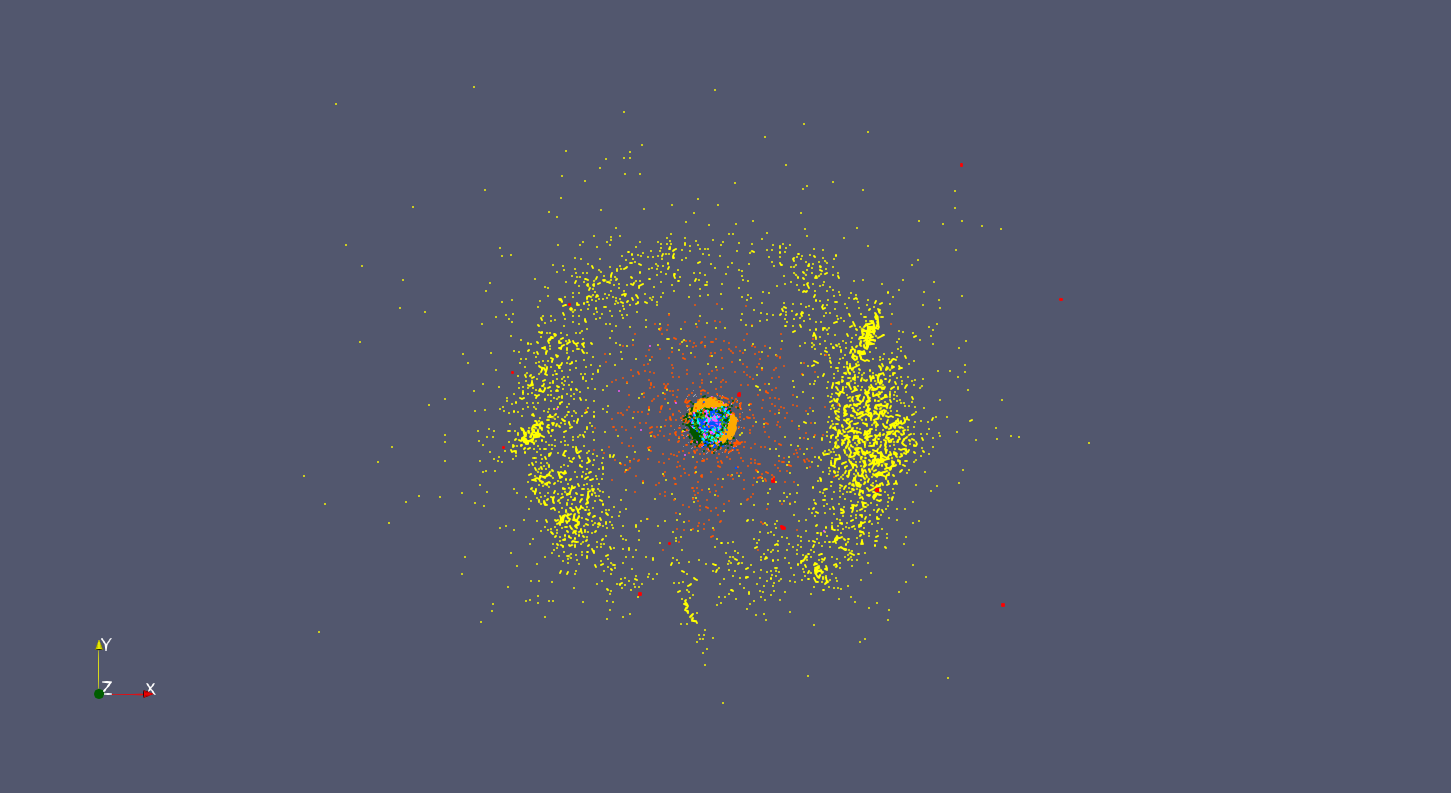
\includegraphics[width=\columnwidth]{figures/all_bodies_whole_system}
	            \caption{\setfontsize{10pt}Our solar system, including outer dwarf planets and TransNeptunian Objects.}
	        \end{figure}
	    \end{column}
	    \hspace*{2em}
	    \begin{column}{.45\linewidth}
	        \begin{figure}
	            \centering
	            \captionsetup{justification=centering}
	            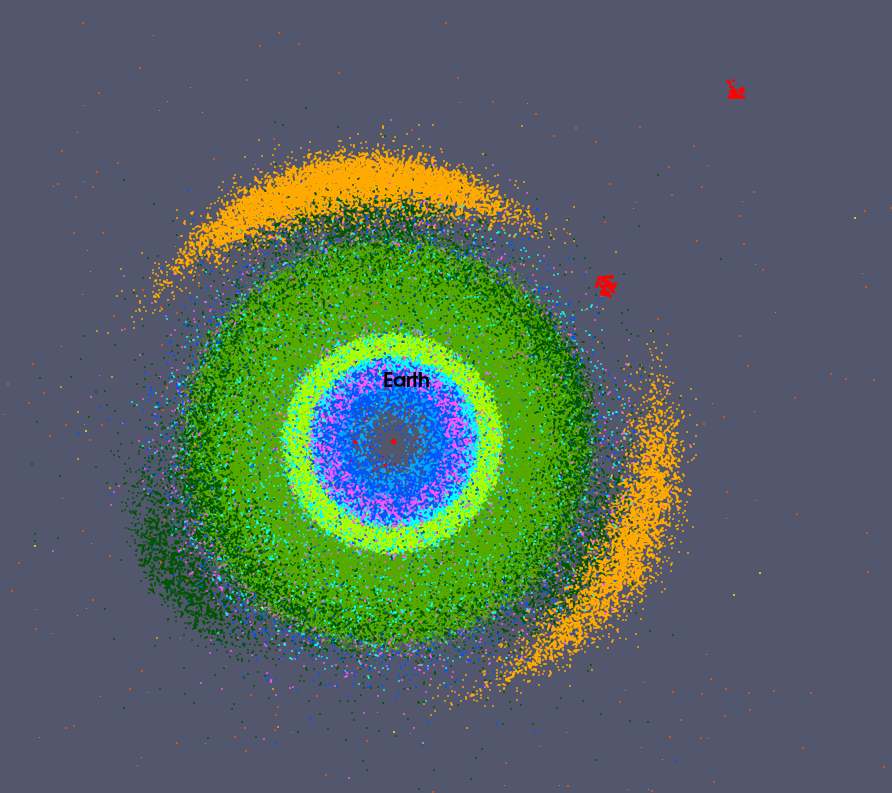
\includegraphics[width=.9\columnwidth]{figures/all_bodies_inner_system}
	            \caption{\setfontsize{10pt}Our solar system zoomed in to Jupiter and the main asteroid belt, Earth highlighted.}
	        \end{figure}
	    \end{column}
	\end{columns}
\end{frame}
%%%%%%%%%%%%%%%%%%%%%%%%%%%%%%%%%%%%%%%%%%%%%%%%%%%%%%%%%%%%%%%%%%%%

%%%%%%%%%%%%%%%%%%%%%%%%%%%%%%%%%%%%%%%%%%%%%%%%%%%%%%%%%%%%%%%%%%%%
\begin{frame}[fragile, c]
  \frametitle{Phase 1: Goal}
  \vspace*{-1em}
  \begin{center}
      Simulation of our solar system: planets, dwarf planets, moons, and asteroids \\(larger than \SI{10}{\kilo\meter}).\\[0.5em]

      \animategraphics[autoplay,loop,controls,width=.76\linewidth]{12}{figures/animation/output-}{0}{253}
  \end{center}
\end{frame}
%%%%%%%%%%%%%%%%%%%%%%%%%%%%%%%%%%%%%%%%%%%%%%%%%%%%%%%%%%%%%%%%%%%%

%%%%%%%%%%%%%%%%%%%%%%%%%%%%%%%%%%%%%%%%%%%%%%%%%%%%%%%%%%%%%%%%%%%%
\begin{frame}[fragile, c]
  \frametitle{Theory: Basic Idea of N-Body Simulations}
  The goal of an n-body simulation is to establish equations of motion for each body.

  \begin{center}
  \vspace*{-1em}
  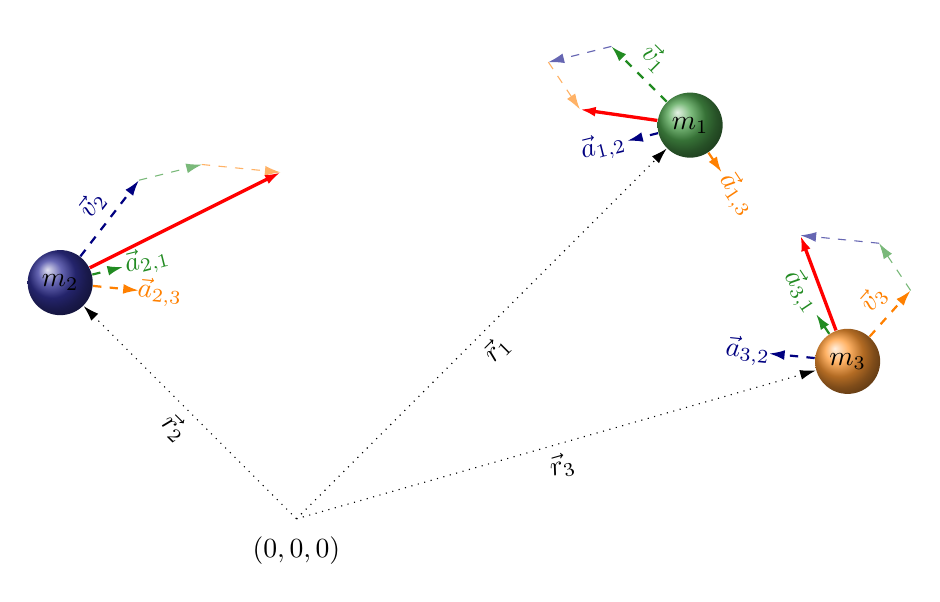
\begin{tikzpicture}
  \coordinate (origo) at (0,0);
  \node[below=0.1 of origo] {$(0, 0, 0)$};

  % body 1
  \node[shading=ball,circle,minimum size=0.5cm,ball color=ForestGreen!80!white] at (5,5) (m1) {$m_1$};
  \draw [dotted,->] (origo) -- (m1) node[midway,sloped,below] {$\vec{r}_1$};
  \draw [dashed,thick,->,ForestGreen] (m1) -- ++(-1,1)  node[midway,sloped,above] {$\vec{v}_1$};
  \draw [dashed,thick,->,NavyBlue] (m1) -- ++(-0.8,-0.2) node[sloped,near end,anchor=east] {$\vec{a}_{1,2}$};
  \draw [dashed,thick,->,orange] (m1) -- ++(0.4,-0.6) node[sloped,near end,anchor=west] {$\vec{a}_{1,3}$};
  \draw [dashed,->,NavyBlue!60] (m1) ++(-1,1)  --  ++(-0.8,-0.2);
  \draw [dashed,->,orange!60] (m1) ++(-1.8,0.8)  --  ++(0.4,-0.6);
  \draw [very thick,->,red] (m1)   --  ++(-1.4,0.2);

  % body 2
  \node[shading=ball,circle,minimum size=0.5cm,ball color=NavyBlue!80!white] at (-3,3) (m2) {$m_2$};
  \draw [dotted,->] (origo) -- (m2) node[midway,sloped,below] {$\vec{r}_2$};
  \draw [dashed,thick,->,NavyBlue] (m2) -- ++(1,1.3)  node[midway,sloped,above] {$\vec{v}_2$};
  \draw [dashed,thick,->,ForestGreen] (m2) -- ++(0.8,0.2) node[sloped,near end,anchor=west] {$\vec{a}_{2,1}$};
  \draw [dashed,thick,->,orange] (m2) -- ++(1,-0.1) node[sloped,near end,anchor=west] {$\vec{a}_{2,3}$};
  \draw [dashed,->,ForestGreen!60] (m2)++(1,1.3) -- ++(0.8,0.2);
  \draw [dashed,->,orange!60] (m2)++(1.8,1.5) -- ++(1,-0.1);
  \draw [very thick,->,red] (m2) -- ++(2.8,1.4);

  % body 3
  \node[shading=ball,circle,minimum size=0.5cm,ball color=orange!80!white] at (7,2) (m3) {$m_3$};
  \draw [dotted,->] (origo) -- (m3) node[midway,sloped,below] {$\vec{r}_3$};
  \draw [dashed,thick,->,orange] (m3) -- ++(0.8,0.9)  node[midway,sloped,above] {$\vec{v}_3$};
  \draw [dashed,thick,->,ForestGreen] (m3) -- ++(-0.4,0.6) node[sloped,near end, anchor=east] {$\vec{a}_{3,1}$};
  \draw [dashed,thick,->,NavyBlue] (m3) -- ++(-1,0.1) node[sloped, near end, anchor=east] {$\vec{a}_{3,2}$};
  \draw [dashed,->,ForestGreen!60] (m3)++(0.8,0.9) -- ++(-0.4,0.6);
  \draw [dashed,->,NavyBlue!60] (m3)++(0.4,1.5) --  ++(-1,0.1);
  \draw [very thick,->,red] (m3) -- ++(-0.6,1.6);
  \end{tikzpicture}
  \end{center}
\end{frame}
%%%%%%%%%%%%%%%%%%%%%%%%%%%%%%%%%%%%%%%%%%%%%%%%%%%%%%%%%%%%%%%%%%%%

%%%%%%%%%%%%%%%%%%%%%%%%%%%%%%%%%%%%%%%%%%%%%%%%%%%%%%%%%%%%%%%%%%%%
\begin{frame}[fragile]
  \frametitle{Theory: Naive Formulation of an N-Body Simulation Problem}
  Each body $i$ with its mass $m_i$ and position vector $\vec{r}_i$ experiences the force $\vec{a}_i$ from all other bodies according to Newton's law of universal gravitation:
  \begin{equation*}
    \vec{a}_i = \sum\limits_{i \neq j} G m_j \frac{\vec{r}_j - \vec{r}_i}{(\norm{\vec{r}_j - \vec{r}_i}_2^2 + \epsilon^2)^\frac{3}{2}}
  \end{equation*}
  \pause
  \vfill
  \begin{itemize}
    \item gravitational constant: $G = \num{6.67430e-11}\frac{\text{m}^3}{\text{kg} \cdot \text{s}^2}$
    \item The physical units of $G$ do not reflect the units used in the data sets.
    \item softening factor: $\epsilon = \num{1e-11}$ to prevent collisions between two bodies
    \item $\norm{}_2^2$: squared Euclidean distance
  \end{itemize}
\end{frame}
%%%%%%%%%%%%%%%%%%%%%%%%%%%%%%%%%%%%%%%%%%%%%%%%%%%%%%%%%%%%%%%%%%%%

%%%%%%%%%%%%%%%%%%%%%%%%%%%%%%%%%%%%%%%%%%%%%%%%%%%%%%%%%%%%%%%%%%%%
\begin{frame}[fragile, label={phase1_requirements}]
  \frametitle{Phase 1: Requirements - Scenario 1}
  Simulating our solar system with the provided planets and moons as well as all asteroids with a \textbf{given} \texttt{diameter} and \texttt{albedo} and where the \textbf{main-belt asteroids} (\texttt{MBA}) are further constraint with a diameter \textbf{greater or equal} than \SI{10}{\kilo\meter} must not take longer than $\SI{1}{\hour}$ on our target system \texttt{simcl1} using $4$ compute nodes:
  \begin{center}
    \setfontsize{6.8pt}
    \mintinline{text}{srun --exclusive -N 4 ./simulate --file scenario1.csv --dt 1h --t_end 12y --vs 2d --vs_dir sim_s1 --theta 1.05}
    \begin{figure}
        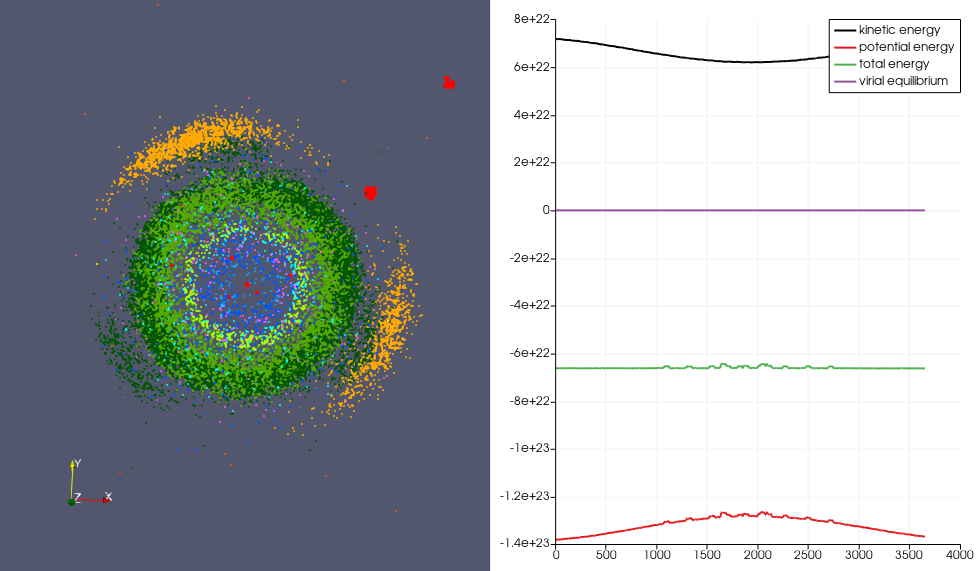
\includegraphics[width=.4\textwidth]{figures/scenario1_result.png}
        \caption{Simulation result of the inner solar system with different colors for the different orbit classes after \num{105192} time steps with \num{19054} bodies.}
    \end{figure}
  \end{center}
\end{frame}
%%%%%%%%%%%%%%%%%%%%%%%%%%%%%%%%%%%%%%%%%%%%%%%%%%%%%%%%%%%%%%%%%%%%

%%%%%%%%%%%%%%%%%%%%%%%%%%%%%%%%%%%%%%%%%%%%%%%%%%%%%%%%%%%%%%%%%%%%
\begin{frame}[fragile]
  \frametitle{Phase 1: Requirements - Scenario 2}
  This time you have \SI{30}{\minute} and again $4$ compute nodes. Try to simulate as many planets, moons, and asteroids as possible for one Earth year!
  \begin{center}
    \setfontsize{6.8pt}
    \mintinline{text}{srun --exclusive -N 4 ./simulate --file scenario2.csv --dt 1h --t_end 1y --vs 7d --vs_dir sim_s2 --theta 1.05} \\[.75em]

    \begin{figure}
        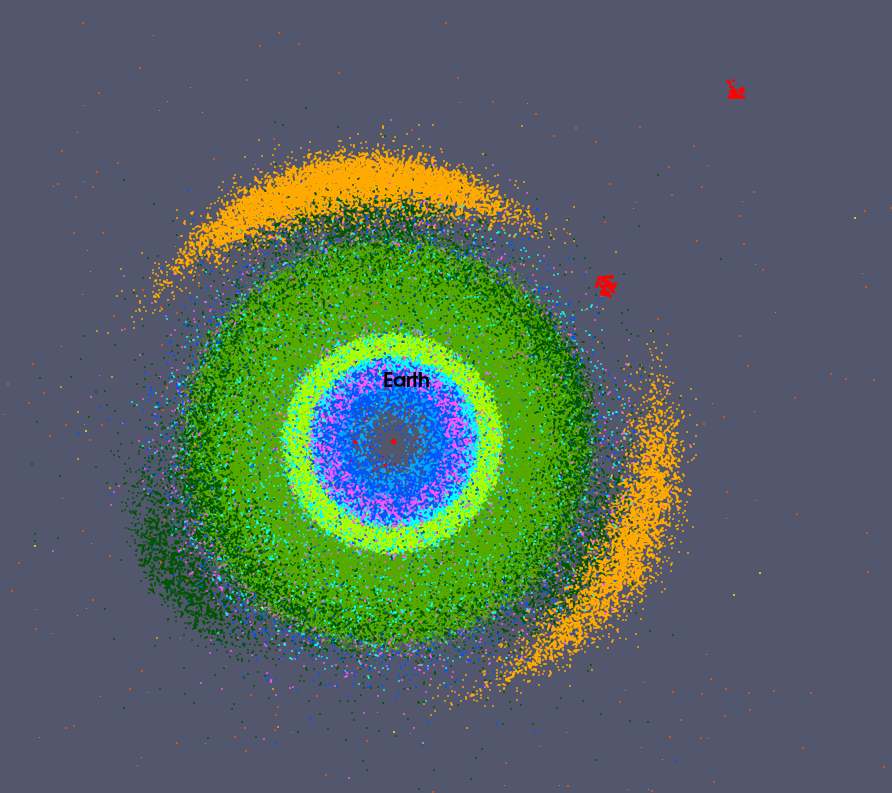
\includegraphics[width=.3\textwidth]{figures/all_bodies_inner_system}
        \caption{Example initial state with \num{1216869} bodies (approximately the maximum number of asteroids in NASA JPL's Small-Body Database).}
    \end{figure}
  \end{center}
\end{frame}
%%%%%%%%%%%%%%%%%%%%%%%%%%%%%%%%%%%%%%%%%%%%%%%%%%%%%%%%%%%%%%%%%%%%

%%%%%%%%%%%%%%%%%%%%%%%%%%%%%%%%%%%%%%%%%%%%%%%%%%%%%%%%%%%%%%%%%%%%
\begin{frame}
    \frametitle{Phase 1: Simulation Data}
    \begin{itemize}
        \item The data sets containing the planets and moons as well as the asteroids for scenario 1 can be found in \link{\urlIliasData}{ILIAS}:
        \item For scenario 2 additional asteroid data can be queried using NASA Jet Propulsion Laboratory's (JPL) \link{https://ssd.jpl.nasa.gov/tools/sbdb_query.html}{Small-Body Database}.
        \item Be aware that some bodies may appear multiple times (e.g., Pluto and its moons) and you have to take care that these bodies are only used once in the actual simulation!

        \item \textbf{Note:} all data is given using the Keplerian orbital elements that must first be converted to Cartesian state vectors.

        \item \textbf{Attention:} The Sun/Sol (with the reference mass \SI{1.98847e30}{\kilo\gram} and epoch $2451544.5$ JD) must always be \textbf{manually} added at the coordinate's origin since it is impossible to specify its orbital elements with respect to itself.

        \item All data must be saved and processed using double precision (FP64, \mintinline{c++}{double}) floating point types.
    \end{itemize}
\end{frame}
%%%%%%%%%%%%%%%%%%%%%%%%%%%%%%%%%%%%%%%%%%%%%%%%%%%%%%%%%%%%%%%%%%%%

%%%%%%%%%%%%%%%%%%%%%%%%%%%%%%%%%%%%%%%%%%%%%%%%%%%%%%%%%%%%%%%%%%%%
\begin{frame}[fragile]
  \frametitle{Phase 1: Submission - \dateDeadlinePhaseOne}
  \begin{itemize}
      \item Submission via \link{\urlIliasSubmissionPhaseOne}{ILIAS}.
      \item Scenario 1: animation of the 3D simulation with a reasonable temporal resolution.
      \item Scenario 2: your custom data set file; the name should contain the number of used bodies.
      \item Scenario 1 \& 2: image of the last time step created via ParaView including an energy plot (kinetic, potential, and total energies) and \texttt{scenario1/2\_save.csv} files with the end states (name, mass, positions, velocities) of the simulations.
      \item The ParaView specific \texttt{.pvd} and \texttt{.vtp} files must \textbf{not} be submitted!
      \item Diagrams with explanations regarding the runtimes (see next slide).
      \item One file, \texttt{submission.sh}, containing the following information (\mintinline{bash}{${}} replaced):
      \begin{minted}[fontsize=\footnotesize]{bash}
#!/bin/sh
git clone ${REPOSITORY_URL} ${GROUP_NAME}
cd ${GROUP_NAME} || exit
git checkout ${COMMIT_HASH}
      \end{minted}

      The commit must contain the code to be evaluated as well as a \texttt{README.md} file describing all necessary steps to build and run your code.

%   \textbf{Note:} it may be more convenient to create a separate git tag for your submission.
  \end{itemize}
\end{frame}
%%%%%%%%%%%%%%%%%%%%%%%%%%%%%%%%%%%%%%%%%%%%%%%%%%%%%%%%%%%%%%%%%%%%

%%%%%%%%%%%%%%%%%%%%%%%%%%%%%%%%%%%%%%%%%%%%%%%%%%%%%%%%%%%%%%%%%%%%
\begin{frame}[fragile]
  \frametitle{Phase 1: Performance Analysis}
  \begin{itemize}
      \item Diagram of the runtimes of the code fixing the number of MPI nodes and OpenMP threads and using different numbers of bodies.
      \item Diagram of the runtimes of the code fixing the number of MPI nodes and varying the number of OpenMP threads (e.g., via \mintinline{bash}{export OMP_NUM_THREADS=N}) for a fixed problem size.
      \item Diagram of the runtimes of the code fixing the number of OpenMP threads and varying the number of MPI nodes for a fixed problem size.
      \item Diagram displaying the runtime and the summed up distances to a very small $\theta$ using different values for $\theta$.
      \item Additional: each diagram must contain a possible \textbf{explanation} for the displayed behavior!
      \item \textbf{Note}: use suitable scenarios for all diagrams.
  \end{itemize}
\end{frame}
%%%%%%%%%%%%%%%%%%%%%%%%%%%%%%%%%%%%%%%%%%%%%%%%%%%%%%%%%%%%%%%%%%%%

%%%%%%%%%%%%%%%%%%%%%%%%%%%%%%%%%%%%%%%%%%%%%%%%%%%%%%%%%%%%%%%%%%%%
\begin{frame}[fragile]
  \frametitle{Phase 1: Competitions}
  Two competitions:
  \begin{itemize}
      \item Which group produces the prettiest simulation animation for scenario 1?
      \begin{itemize}
          \item How to best display the vastly different body sizes in ParaView?
          \item Added body textures?
          \item Camera movement?
      \end{itemize}
      \item Which group can simulate the most bodies in the available time? (scenario 2)
      \begin{itemize}
          \item Add your runtime and number of bodies to the \link{\urlNextcloud}{Nextcloud table}% using the password \texttt{\passwordNextcloud}.
          \item At the end of phase 1, the runtimes and number of bodies will be verified by us.
          \item Real simulation without tricks (e.g., it is \textbf{not} allowed to simply output pre-calculated time steps!).
      \end{itemize}
  \end{itemize}
    \vfill
  \itFollows{The winners of each competition will receive a small reward!}
\end{frame}
%%%%%%%%%%%%%%%%%%%%%%%%%%%%%%%%%%%%%%%%%%%%%%%%%%%%%%%%%%%%%%%%%%%%

\section*{Phase 2}
%%%%%%%%%%%%%%%%%%%%%%%%%%%%%%%%%%%%%%%%%%%%%%%%%%%%%%%%%%%%%%%%%%%%
\begin{frame}
	\frametitle{Phase 2: Goal}
    \vspace*{-0.2cm}
    \visible<2->{
    \begin{tikzpicture}[overlay]
        \node at (2.9, -.55) {
\includegraphics[width=2.85cm]{figures/phase_2_intro/HPX_STELLAR_blue.png}\tiny[1]};

        \begin{scope}[scale=.8, shift={(0, -1.5)}]
            \node (gpu) at (2, -1.5) {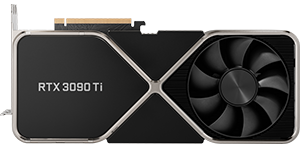
\includegraphics[width=3.5cm]{figures/phase_2_intro/nvidia-geforce-rtx-3090-ti.png}\tiny[2]};

            \node (cuda) at (0.5, -3.75) {
\includegraphics[width=1.2cm]{figures/phase_2_intro/Nvidia_CUDA_Logo.jpg}};
            \node (sycl) at (3.5, -3.75) {
\includegraphics[width=1.5cm]{figures/phase_2_intro/sycl_logo.png}};
            \node (opencl) at (2, -4.5) {
\includegraphics[width=1.5cm]{figures/phase_2_intro/OpenCL_logo.svg.png}};

            \draw[dashed, -latex] (gpu) -- (cuda);
            \draw[dashed, -latex] (gpu) -- (sycl);
            \draw[dashed, -latex] (gpu) -- (opencl);
        \end{scope}
        \node at (11.75, 0) {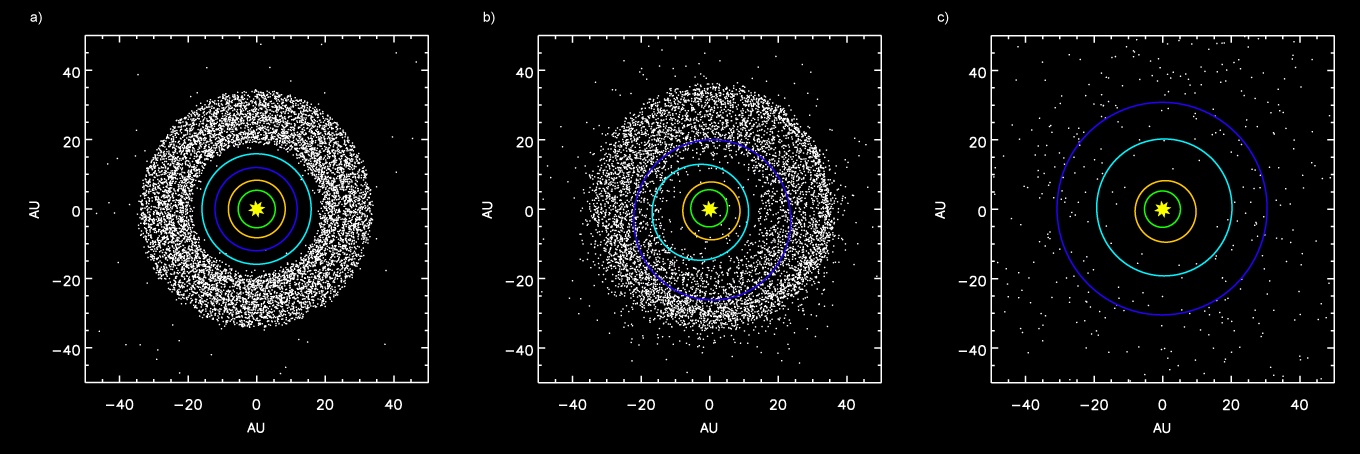
\includegraphics[width=6cm]{figures/phase_2_intro/nice_model.png}\,\tiny[3]};
        \node at (11.5, -3.25) {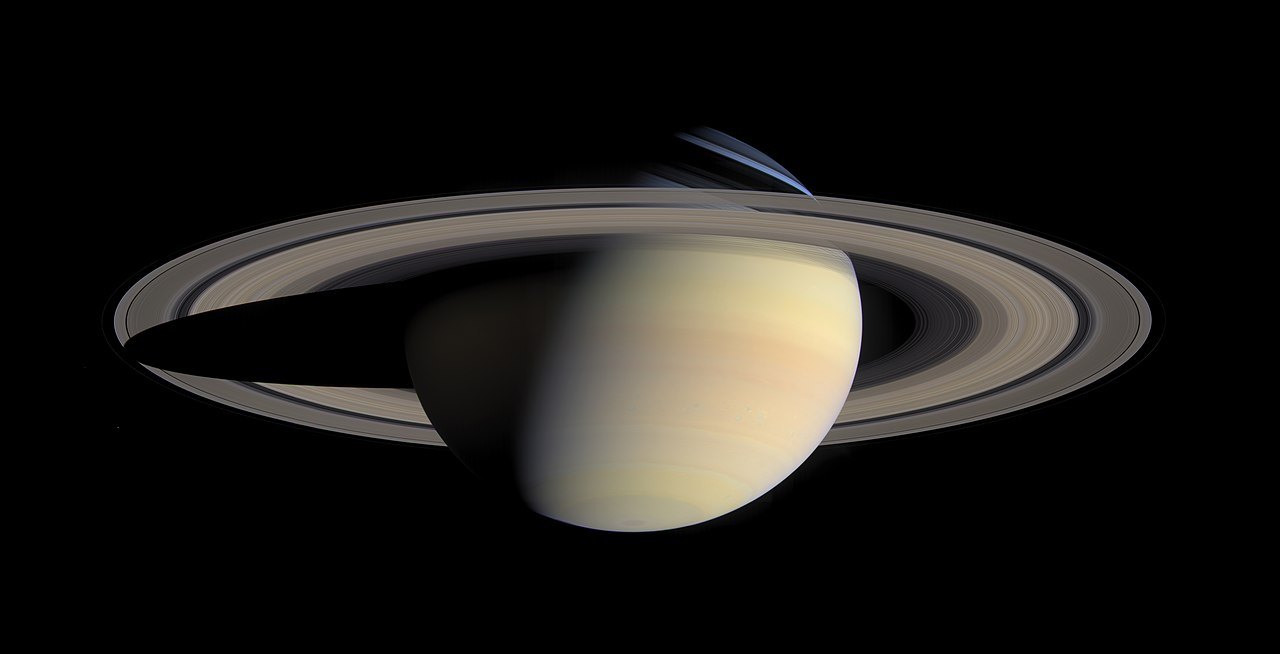
\includegraphics[width=5cm]{figures/phase_2_intro/1280px-Saturn_from_Cassini_Orbiter_(2004-10-06).jpeg}\,\tiny[4]};
    \end{tikzpicture}
    }

	\vspace*{-2.5cm}
	\begin{center}
	    \bfseries \setfontsize{150pt}%
	    ?
	\end{center}


	\btVFill
	\centering
    \vspace*{3em}
	\DisplayRightArrow Everyone can do a custom project on his own based on the code of phase 1.
	\vspace{-.25em}
	\visible<2->{
    	\begin{flushleft}
        \tiny Image Sources: \\
    	\tiny [1]: \url{https://hpx-docs.stellar-group.org/latest/html/index.html} \\
    	\tiny [2]: \url{https://store.nvidia.com/de-de/geforce/store/?page=1&limit=9&locale=de-de} \\
    	\tiny [3]: \url{https://en.wikipedia.org/wiki/Nice_model} \\
    	\tiny [4]: \url{https://en.wikipedia.org/wiki/Saturn}
    	\end{flushleft}
	}
\end{frame}
%%%%%%%%%%%%%%%%%%%%%%%%%%%%%%%%%%%%%%%%%%%%%%%%%%%%%%%%%%%%%%%%%%%%

%%%%%%%%%%%%%%%%%%%%%%%%%%%%%%%%%%%%%%%%%%%%%%%%%%%%%%%%%%%%%%%%%%%%
\begin{frame}
	\frametitle{Phase 2: Goal}
	Extend your code of phase 1 by an individual project, possible examples are:
	\begin{itemize}
	    \item code acceleration using GPUs (e.g., via CUDA, OpenCL, Kokkos, or SYCL)
	    \item replacing MPI with another framework for distributed computing like HPX
	    \item add more physics (e.g., collision detection for simulating the Kessler syndrome)
	    \item implementing more efficient algorithms (e.g., Fast Multipole Methods)
	    \item lifting the simplification that every node saves all bodies \\
	    $\rightarrow$ each node only knows about a subset of all bodies (needs load balancing)
	    \item new simulation scenarios (e.g., close-up simulation of Saturn including its rings, the Oort Cloud with Nemesis, the Nice model, or the \enquote{galaxy far, far away})
	    \item $\dots$
	\end{itemize}
	\begin{center}
	    \textbf{Restrictions:} It must have something to do with our overall parallelism topic and it must be different from your group members' projects!
	\end{center}
	\btVFill
	\itFollows{Each project must be approved by us, i.e., simply send us an email with 2-3 sentences describing your idea before you start working on it.}
\end{frame}
%%%%%%%%%%%%%%%%%%%%%%%%%%%%%%%%%%%%%%%%%%%%%%%%%%%%%%%%%%%%%%%%%%%%

%%%%%%%%%%%%%%%%%%%%%%%%%%%%%%%%%%%%%%%%%%%%%%%%%%%%%%%%%%%%%%%%%%%%
\begin{frame}[fragile]
  \frametitle{Phase 2: Submission - \dateDeadlinePhaseTwo}
  \begin{itemize}
      \item Submission via \link{\urlIliasSubmissionPhaseTwo}{ILIAS}.
      \item A \texttt{submission.sh} file as for \hyperref[phase1_requirements]{phase 1} with adjusted placeholders and commit hash.
      \item A \texttt{.pdf} describing your project idea, implementation, and possible results on \textbf{at least} 5 pages excluding the title page and possible references
      \item All supplementary files for your individual project (e.g., simulation data sets for a new scenario or new runtime diagrams).
      \item The \link{\urlIliasLatexTemplate}{\LaTeX\xspace template} can be found in ILIAS.
  \end{itemize}
\end{frame}
%%%%%%%%%%%%%%%%%%%%%%%%%%%%%%%%%%%%%%%%%%%%%%%%%%%%%%%%%%%%%%%%%%%%

%%%%%%%%%%%%%%%%%%%%%%%%%%%%%%%%%%%%%%%%%%%%%%%%%%%%%%%%%%%%%%%%%%%%
\begin{frame}[fragile]
  \frametitle{Phase 2: Presentation - \dateFinal}
  \begin{itemize}
    \item $15$-$\SI{20}{\minute}$ presentation + $\SI{5}{\minute}$ Q\&A per student.
    \item The slides must be uploaded in \link{\urlIliasSubmissionFinal}{ILIAS}.
    \item Phase 2 will be the crucial part for your grade where this presentation is a major part of! The results from phase 1 play only a minor role in grading!
    \vspace*{1em}
    \item The slides should contain all your results of phase 2.
    \item They should also contain the problems you encountered during phase 2.
  \end{itemize}
\end{frame}
%%%%%%%%%%%%%%%%%%%%%%%%%%%%%%%%%%%%%%%%%%%%%%%%%%%%%%%%%%%%%%%%%%%%

\section*{General Remarks}
%%%%%%%%%%%%%%%%%%%%%%%%%%%%%%%%%%%%%%%%%%%%%%%%%%%%%%%%%%%%%%%%%%%%
\begin{frame}[fragile]
  \frametitle{General Submission Guidelines}
  \begin{itemize}
    \item For each phase \textbf{exactly} one \texttt{*.zip} or \texttt{*.tar.gz} archive must be uploaded to \link{\urlIliasCourse}{ILIAS} with the content corresponding to the respective phase.
    \item PhasePhasenumber followed by the family name (of all group members), e.g., \texttt{Phase1\_Name1\_Name2\_Name3.tar.gz}.
    \item Each file in the archive must contain the name (of \textbf{all} group members).
    \item The submission must be compilable and executable on a normal Linux command line on one of our machines, i.e., no IDE specific build scripts are allowed!
  \end{itemize}
\end{frame}
%%%%%%%%%%%%%%%%%%%%%%%%%%%%%%%%%%%%%%%%%%%%%%%%%%%%%%%%%%%%%%%%%%%%

%%%%%%%%%%%%%%%%%%%%%%%%%%%%%%%%%%%%%%%%%%%%%%%%%%%%%%%%%%%%%%%%%%%%
\begin{frame}
  \frametitle{GitLab}
  \begin{itemize}
    \item After applying for our hardware and receiving an account, this account can also be used to login to our \link{https://gitlab-sim.informatik.uni-stuttgart.de}{GitLab server}.
    \item For phase 1, you get one private repository per submission group, for phase 2, one fork of the phase 1 repository per student.
    \item Each repository \textbf{must} have one \texttt{README} file containing all necessary information on how to compile and execute your code.
    \item An \link{https://github.com/SCTeaching-NBody/LabCourse_Template}{example \texttt{C++ \& CMake} repository} with small MPI + OpenMP code snippets can also be found in our GitLab.
  \end{itemize}
\end{frame}
%%%%%%%%%%%%%%%%%%%%%%%%%%%%%%%%%%%%%%%%%%%%%%%%%%%%%%%%%%%%%%%%%%%%

%%%%%%%%%%%%%%%%%%%%%%%%%%%%%%%%%%%%%%%%%%%%%%%%%%%%%%%%%%%%%%%%%%%%
\begin{frame}{CI via GitLab}

\begin{itemize}
    \item You should at least have 10 useful test cases and a test coverage of at least \SI{80}{\percent}!
    \item Install a GitLab runner on your machine and register a runner for your repository/fork.
    \begin{itemize}
        \item \link{https://docs.gitlab.com/runner/install/}{Install instructions} for a GitLab runner.
        \item GitLab runner as docker service as shown in the \link{https://github.com/Simulation-Software-Engineering/Lecture-Material/blob/main/05_testing_and_ci/gitlab_ci_demo.md}{SSE lecture}.
        \item The runner should support the docker executor and should be able to run Linux images.
    \end{itemize}
    \item Add a GitLab pipeline status badge to the project that is based on your pipeline and the main branch.
\end{itemize}

If you cannot add such a runner on your machine, please email one of us with the registration token and your GitLab username. We will then add a runner to your repository.

\end{frame}
%%%%%%%%%%%%%%%%%%%%%%%%%%%%%%%%%%%%%%%%%%%%%%%%%%%%%%%%%%%%%%%%%%%%

%%%%%%%%%%%%%%%%%%%%%%%%%%%%%%%%%%%%%%%%%%%%%%%%%%%%%%%%%%%%%%%%%%%%
\begin{frame}[fragile]
  \frametitle{Allowed Software}
  \begin{itemize}
      \item You are allowed to use any third-party library that does \textbf{not} solve a significant part of your project (like converting the orbital elements to state vectors, performing the actual simulation, writing the ParaView output, etc.).
      \item If you are not sure if you are allowed to use a library, feel free to contact us via email or ILIAS.
      \item Utility libraries, however, are allowed and we recommend the usage of the following:
      \begin{itemize}
          \item any command line parser library (e.g., \link{https://github.com/jarro2783/cxxopts}{\texttt{cxxopts}})
          \item the \texttt{C++} formatting library \link{https://github.com/fmtlib/fmt}{\texttt{\{fmt\}}}
      \end{itemize}
      \item \textbf{Note:} you \textbf{must} provide installation instructions for every library you use! Or better use something like CMake's \mintinline{text}{FetchContent_Declare} to install it if possible automatically.
      \item Another way to install third-party libraries without the need for root privileges is \link{https://github.com/spack/spack}{\texttt{spack}}.
      \item Any \texttt{C++} standard from \texttt{C++17} and upwards is allowed.
  \end{itemize}
\end{frame}
%%%%%%%%%%%%%%%%%%%%%%%%%%%%%%%%%%%%%%%%%%%%%%%%%%%%%%%%%%%%%%%%%%%%

%%%%%%%%%%%%%%%%%%%%%%%%%%%%%%%%%%%%%%%%%%%%%%%%%%%%%%%%%%%%%%%%%%%%
\begin{frame}[fragile]
  \frametitle{General Recommendations and Remarks}
  \begin{itemize}
    \item Your simulation should include some sort of progress indication (e.g., a terminal output each \SI{10}{\percent} of the simulation).
    \item Use a \texttt{C++} IDE (e.g., Visual Studio (Code) or CLion) and their tools like profiler, debugger, auto-formatting, linter, etc.
    \item Use an automated build system, preferable \link{https://cmake.org/}{CMake}.
    \item Document your code (for you \textbf{and} for us!), e.g., via \link{https://doxygen.nl/}{Doxygen}.
    \item The installation and usage of your program as well as its verification should be as easy as possible.
    \item Test your program on our target Linux system \texttt{simcl1}.
    \item One of the main goals of this lab course is to encourage working independently, however, if questions arise, feel free to ask them in the \link{\urlIliasForumGeneral}{ILIAS forum}.
    \item The easiest way to determine the total runtime of your code is to use the Linux \mintinline{bash}{time} utility: \mintinline{bash}{time ./simulate --file data.csv --dt 1h --t_end 1y --vs 2d --theta 1.05}
    \item Start to work on phase 1 and phase 2 soon enough!
    \item Secret tip: MIT's \link{https://missing.csail.mit.edu/}{\enquote{The Missing Semester of Your CS Education}}
  \end{itemize}
\end{frame}
%%%%%%%%%%%%%%%%%%%%%%%%%%%%%%%%%%%%%%%%%%%%%%%%%%%%%%%%%%%%%%%%%%%%

%%%%%%%%%%%%%%%%%%%%%%%%%%%%%%%%%%%%%%%%%%%%%%%%%%%%%%%%%%%%%%%%%%%%
\begin{frame}[fragile]
	\frametitle{Time-Management Phase 1: 4 Weeks 6 Days}
	\begin{itemize}
		\item Think about a suitable time schedule: \textbf{when} should we implement \textbf{what}.
		\item For a successful Phase 1, we suggest the following rough schedule:
		\begin{description}
			%\setlength\itemsep{.4em}
			\item[1st week] project-setup, IO, and conversion from keplerian orbital elements to cartesian state vectors
			\item[2nd week] implement the naive approach to get familiar with the n-body problem (not needed for the final submission)
			\item
			\item[meeting]
			\item
			\item[3rd week] implement the Barnes-Hut algorithm
			\item[4th week] paralleize your implementation using MPI + OpenMP
			\item
			\item[meeting]
			\item
			\item[5th week] further optimize and benchmark your code
		\end{description}
	\end{itemize}
	
\end{frame}
%%%%%%%%%%%%%%%%%%%%%%%%%%%%%%%%%%%%%%%%%%%%%%%%%%%%%%%%%%%%%%%%%%%%

%%%%%%%%%%%%%%%%%%%%%%%%%%%%%%%%%%%%%%%%%%%%%%%%%%%%%%%%%%%%%%%%%%%%
\begin{frame}{On a Final Note}
    \begin{center}
        \Large\bfseries\itshape
        The simulation is greatly simplified!
    \end{center}
    \pause
    \vfill
    Many physical effects or properties are ignored or only roughly estimated:
    \begin{itemize}
        \item rotational forces, tidal forces, radiation, magnetic fields, etc.
        \item various value approximations, mainly for the asteroids' masses
        \item shape of the body (assumed to be spherical)
        \item $\dots$
    \end{itemize}
    \pause
    \vfill
    \itFollows{Nevertheless, it is good enough for a stable simulation of the whole of our solar system including the sun, planets, dwarf planets, moons, and major asteroids!}
\end{frame}
%%%%%%%%%%%%%%%%%%%%%%%%%%%%%%%%%%%%%%%%%%%%%%%%%%%%%%%%%%%%%%%%%%%%

%%%%%%%%%%%%%%%%%%%%%%%%%%%%%%%%%%%%%%%%%%%%%%%%%%%%%%%%%%%%%%%%%%%%
\begin{frame}[label={important_deadlines}]
  \frametitle{Important Deadlines}

  \begin{description}
    \item[\dateKickoffPhaseOne] Kick-off
    \item[\dateDeadlinePhaseZero] Deadline Group Formation
    \item[\dateDeadlinePhaseOne] Deadline Phase 1
    \item[\dateDeadlinePhaseTwo] Deadline Phase 2
    \item[\dateFinal] Final Presentations% (possibly on more than one day)
  \end{description}
  \vfill
  \itFollows{\textbf{Do not} forget to register for our lab course in \link{https://campus.uni-stuttgart.de}{C@MPUS}!}
%   \todo{(zwei-)wöchentliche Treffen?}
\end{frame}
%%%%%%%%%%%%%%%%%%%%%%%%%%%%%%%%%%%%%%%%%%%%%%%%%%%%%%%%%%%%%%%%%%%%



%%%%%%%%%%%%%%%%%%%%%%%%%%%%%%%%%%%%%%%%%%%%%%%%%%%%%%%%%%%%%%%%%%%%
\appendix
{
\usebackgroundtemplate{\transparent{0.35}\includegraphics[width=\paperwidth]{figures/backgrounds/bonus_material}}
\begin{frame}
    \vspace{1.5cm}
    \begin{center}
        \setfontsize{35pt}\bfseries
        Bonus Material
    \end{center}
    \btVFill
    \setbeamertemplate{section in toc}{\raggedright \leftskip=1.6em \parindent=-1.6em \textcolor{structure.fg}{$\blacktriangleright$}\hspace{.5em}~\inserttocsection\\}
    \begin{multicols}{2}
        \tableofcontents[subsectionstyle=hide]
    \end{multicols}
\end{frame}
}
%%%%%%%%%%%%%%%%%%%%%%%%%%%%%%%%%%%%%%%%%%%%%%%%%%%%%%%%%%%%%%%%%%%%

%%% input all bonus material content slides
\section{Target System}
%%%%%%%%%%%%%%%%%%%%%%%%%%%%%%%%%%%%%%%%%%%%%%%%%%%%%%%%%%%%%%%%%%%%
\begin{frame}
  \frametitle{Target System: \texttt{simcl1} - Hardware}
  \texttt{simcl1} is a small cluster consisting of one login node and $\num{4}$ compute nodes. \\
  \textbf{Attention:} \textbf{do not} perform \textbf{any} calculations on the login node!
  \vfill
  Available hardware per compute node:
  \begin{itemize}
      \item $\num{1}$ \link{https://www.amd.com/en/products/cpu/amd-epyc-9274f}{AMD EPYC 9274F 24-Core @ 
4.05GHz}
      \begin{itemize}
          \item $\num{48}$ physical cores
          \item $\num{96}$ hyper threads
          \item $\num{2}$ sockets
      \end{itemize}
      \item $\SI{384}{\gibi\byte}$ DDR5 RAM
      \item $\SI{1.5}{\tera\byte}$ \texttt{/data/scratch} space (\textbf{not shared} across nodes of the cluster)\\
      \itFollows{If you want to use the \texttt{/scratch} space instead of your \texttt{\$HOME} directory, you must create the \texttt{/data/scratch/FaPra/\$\{GROUP\_NAME\}} custom directory and delete it afterwards!}
      \item inter-node connection via \SI{10}{\giga\byte} Ethernet
      \item nodes 1 and 2 contain an NVIDIA A30 GPU each
      \item node 3 contains an AMD Mi210 GPU
  \end{itemize}
\end{frame}
%%%%%%%%%%%%%%%%%%%%%%%%%%%%%%%%%%%%%%%%%%%%%%%%%%%%%%%%%%%%%%%%%%%%

\subsection{Connecting to simcl1}
%%%%%%%%%%%%%%%%%%%%%%%%%%%%%%%%%%%%%%%%%%%%%%%%%%%%%%%%%%%%%%%%%%%%
\begin{frame}[fragile]{Target System: \texttt{simcl1} - Connecting to the Cluster - 1}
    First login to our server:
    \begin{enumerate}
        \item \mintinline{sh}{ssh ${USERNAME}@ipvslogin.informatik.uni-stuttgart.de}
        \item You will be prompted to input your password.
        \item Change your initial password: See \mintinline{sh}{passwd} and follow the displayed instructions. This \textbf{must} be done during your first login.
        \item Disconnect from the server by either typing \mintinline{sh}{exit} or using \texttt{Strg + d}.
    \end{enumerate}
    \pause
    \vfill
    Connecting to the \texttt{simcl1} cluster's login node using an ssh key:
    \begin{enumerate}
        \item \link{https://docs.oracle.com/en/cloud/cloud-at-customer/occ-get-started/generate-ssh-key-pair.html}{Generate a new ssh key pair} (if none already exists).
        \item Copy your public ssh key to our login server via:
        {
            \setfontsize{9pt}
            \mintinline{sh}{ssh-copy-id -i ~/.ssh/id_rsa ${USERNAME}@ipvslogin.informatik.uni-stuttgart.de}
        }
        \textbf{Note:} you will be prompted to enter your passwords.
    \end{enumerate}
\end{frame}
%%%%%%%%%%%%%%%%%%%%%%%%%%%%%%%%%%%%%%%%%%%%%%%%%%%%%%%%%%%%%%%%%%%%

%%%%%%%%%%%%%%%%%%%%%%%%%%%%%%%%%%%%%%%%%%%%%%%%%%%%%%%%%%%%%%%%%%%%
\begin{frame}[fragile]{Target System: \texttt{simcl1} - Connecting to the Cluster - 2}
    \begin{enumerate}
        \setcounter{enumi}{2}
        \item Add the following lines to your \texttt{\~{}/.ssh/config} file (on your local machine):\vspace*{-.5em}
        \begin{minted}{bash}
host ipvslogin
    ForwardAgent yes
    hostname ipvslogin.informatik.uni-stuttgart.de
    user ${USERNAME}
    IdentityFile ~/.ssh/id_rsa

host simcl1
    ForwardAgent yes
    ProxyJump ipvslogin
    hostname
    user ${USERNAME}
    IdentityFile ~/.ssh/id_rsa
        \end{minted}
        \item Now you can login to \texttt{simcl1} by simply using: \mintinline{sh}{ssh simcl1}
    \end{enumerate}
\end{frame}
%%%%%%%%%%%%%%%%%%%%%%%%%%%%%%%%%%%%%%%%%%%%%%%%%%%%%%%%%%%%%%%%%%%%

\section{SLURM}
%%%%%%%%%%%%%%%%%%%%%%%%%%%%%%%%%%%%%%%%%%%%%%%%%%%%%%%%%%%%%%%%%%%%
\begin{frame}{SLURM Workload Manager}
    The most important SLURM commands are:
    %\setbeamertemplate{description item}[align left]
    \begin{description}[ ]
      \item[\mintinline{text}{sinfo}]\hfill\\ \quad
      list available nodes including their operational state
      \item[\mintinline{text}{squeue}]\hfill\\\quad
      list running or pending jobs
      \item[\mintinline{text}{scancel JOB_ID}]\hfill\\\quad
      cancel to job identified by \texttt{JOB\_ID} and remove it from the queue
      \item[\mintinline{text}{srun --pty bash}]\hfill\\\quad
      start an interactive session on one node
      \item[\mintinline{text}{srun -N X ./simulate [OPTIONS]}]\hfill\\\quad
      run your simulation on $X$ compute nodes in parallel
      \item[\mintinline{text}{sbatch -N X -n X --wrap "./simulate [OPTIONS]"}]\hfill\\\quad
      queue your simulation on $X$ compute nodes in parallel for future execution
    \end{description}
    For more information, e.g., using \mintinline{text}{sbatch} with a script instead of \mintinline{text}{--wrap}, see the official \link{https://slurm.schedmd.com/}{SLURM homepage}.
\end{frame}
%%%%%%%%%%%%%%%%%%%%%%%%%%%%%%%%%%%%%%%%%%%%%%%%%%%%%%%%%%%%%%%%%%%%
\section{Theory}
%%%%%%%%%%%%%%%%%%%%%%%%%%%%%%%%%%%%%%%%%%%%%%%%%%%%%%%%%%%%%%%%%%%%
\begin{frame}[fragile, c]
  \frametitle{Theory: Basic Idea of N-Body Simulations}
  The goal of an n-body simulation is to establish equations of motion for each body.
  
  \begin{center}
  \vspace*{-1em}
  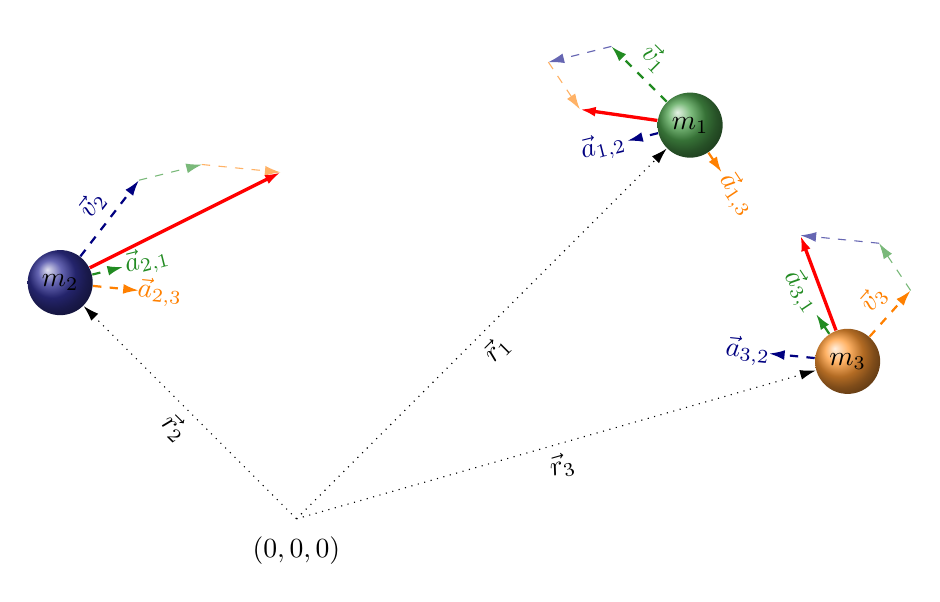
\begin{tikzpicture}
  \coordinate (origo) at (0,0);
  \node[below=0.1 of origo] {$(0, 0, 0)$};
  
  % body 1
  \node[shading=ball,circle,minimum size=0.5cm,ball color=ForestGreen!80!white] at (5,5) (m1) {$m_1$};
  \draw [dotted,->] (origo) -- (m1) node[midway,sloped,below] {$\vec{r}_1$};
  \draw [dashed,thick,->,ForestGreen] (m1) -- ++(-1,1)  node[midway,sloped,above] {$\vec{v}_1$};
  \draw [dashed,thick,->,NavyBlue] (m1) -- ++(-0.8,-0.2) node[sloped,near end,anchor=east] {$\vec{a}_{1,2}$};
  \draw [dashed,thick,->,orange] (m1) -- ++(0.4,-0.6) node[sloped,near end,anchor=west] {$\vec{a}_{1,3}$};
  \draw [dashed,->,NavyBlue!60] (m1) ++(-1,1)  --  ++(-0.8,-0.2);
  \draw [dashed,->,orange!60] (m1) ++(-1.8,0.8)  --  ++(0.4,-0.6);
  \draw [very thick,->,red] (m1)   --  ++(-1.4,0.2);
  
  % body 2
  \node[shading=ball,circle,minimum size=0.5cm,ball color=NavyBlue!80!white] at (-3,3) (m2) {$m_2$};
  \draw [dotted,->] (origo) -- (m2) node[midway,sloped,below] {$\vec{r}_2$};
  \draw [dashed,thick,->,NavyBlue] (m2) -- ++(1,1.3)  node[midway,sloped,above] {$\vec{v}_2$};
  \draw [dashed,thick,->,ForestGreen] (m2) -- ++(0.8,0.2) node[sloped,near end,anchor=west] {$\vec{a}_{2,1}$};
  \draw [dashed,thick,->,orange] (m2) -- ++(1,-0.1) node[sloped,near end,anchor=west] {$\vec{a}_{2,3}$};
  \draw [dashed,->,ForestGreen!60] (m2)++(1,1.3) -- ++(0.8,0.2);
  \draw [dashed,->,orange!60] (m2)++(1.8,1.5) -- ++(1,-0.1);
  \draw [very thick,->,red] (m2) -- ++(2.8,1.4);
  
  % body 3
  \node[shading=ball,circle,minimum size=0.5cm,ball color=orange!80!white] at (7,2) (m3) {$m_3$};
  \draw [dotted,->] (origo) -- (m3) node[midway,sloped,below] {$\vec{r}_3$};
  \draw [dashed,thick,->,orange] (m3) -- ++(0.8,0.9)  node[midway,sloped,above] {$\vec{v}_3$};
  \draw [dashed,thick,->,ForestGreen] (m3) -- ++(-0.4,0.6) node[sloped,near end, anchor=east] {$\vec{a}_{3,1}$};
  \draw [dashed,thick,->,NavyBlue] (m3) -- ++(-1,0.1) node[sloped, near end, anchor=east] {$\vec{a}_{3,2}$};
  \draw [dashed,->,ForestGreen!60] (m3)++(0.8,0.9) -- ++(-0.4,0.6);
  \draw [dashed,->,NavyBlue!60] (m3)++(0.4,1.5) --  ++(-1,0.1);
  \draw [very thick,->,red] (m3) -- ++(-0.6,1.6);
  \end{tikzpicture}
  \end{center}
\end{frame}
%%%%%%%%%%%%%%%%%%%%%%%%%%%%%%%%%%%%%%%%%%%%%%%%%%%%%%%%%%%%%%%%%%%%

%%%%%%%%%%%%%%%%%%%%%%%%%%%%%%%%%%%%%%%%%%%%%%%%%%%%%%%%%%%%%%%%%%%%
\begin{frame}[fragile]
  \frametitle{Theory: Naive Formulation of an N-Body Simulation Problem}
  Each body $i$ with its mass $m_i$ and position vector $\vec{r}_i$ experiences the force $\vec{a}_i$ from all other bodies according to Newton's law of universal gravitation:
  \begin{equation*}
    \vec{a}_i = \sum\limits_{i \neq j} G m_j \frac{\vec{r}_j - \vec{r}_i}{(\norm{\vec{r}_j - \vec{r}_i}_2^2 + \epsilon^2)^\frac{3}{2}}
  \end{equation*}
  \pause
  \begin{itemize}
    \item gravitational constant: $G = \num{6.67430e-11}\frac{\text{m}^3}{\text{kg} \cdot \text{s}^2}$
    \item The physical units of $G$ do not reflect the units used in the data sets:
          \begin{itemize}
            \item distance in astronomical units:  $\SI{1}{\au} = \SI{1.49597870691e+11}{\meter}$
            \item time in days: $\SI{1}{\day} = \SI{86400}{\second}$
          \end{itemize}
    \item \textbf{Note:} the correctly scaled $G$ should be calculate in your program!
    \item softening factor: $\epsilon = \num{1e-11}$ to prevent collisions between two bodies
    \item $\norm{}_2^2$: squared Euclidean distance
  \end{itemize}
\end{frame}
%%%%%%%%%%%%%%%%%%%%%%%%%%%%%%%%%%%%%%%%%%%%%%%%%%%%%%%%%%%%%%%%%%%%

%%%%%%%%%%%%%%%%%%%%%%%%%%%%%%%%%%%%%%%%%%%%%%%%%%%%%%%%%%%%%%%%%%%%
\begin{frame}[fragile]
  \frametitle{Theory: Energy of the System}
  \begin{itemize}
    \item kinetic energy: $E_K = \sum\limits_{i}\frac{1}{2} m_i \norm{\vec{v}_i}_2^2$
    \item potential energy: $E_P = -\sum\limits_{i < j} \frac{G m_i m_j}{\norm{\vec{r}_j - \vec{r}_i}_2}$
    \item sum of the energies in the system: $E_T = E_K + E_P$\vspace{.7em}
    \item $E_T$ must be \enquote{constant} in a stable simulation (conservation of energy)!
  \end{itemize}
  \vfill
  \pause
  The Virial Equilibrium:
  
  $$ \frac{2 \cdot E_K}{\abs{E_P}} \approx 1.0 $$
  
  as a dynamic equilibrium state on a timescale comparable to a few times the typical time needed for a body to cross the system.
  \vfill
  \textbf{Question:} What happens if the result is $> 1.0$ or $< 1.0$?
  
  \vfill
  \setfontsize{8pt}
  See: \url{http://www.scholarpedia.org/article/N-body_simulations_(gravitational)}
\end{frame}
%%%%%%%%%%%%%%%%%%%%%%%%%%%%%%%%%%%%%%%%%%%%%%%%%%%%%%%%%%%%%%%%%%%%

\subsection{Barnes-Hut}
%%%%%%%%%%%%%%%%%%%%%%%%%%%%%%%%%%%%%%%%%%%%%%%%%%%%%%%%%%%%%%%%%%%%
\begin{frame}[fragile]
  \frametitle{Theory: Barnes-Hut Algorithm to Speed Up the Simulation}
  Combine bodies that are far enough away from pseudo-bodies to reduce the number of necessary force calculations.
  \vfill
  \begin{center}
  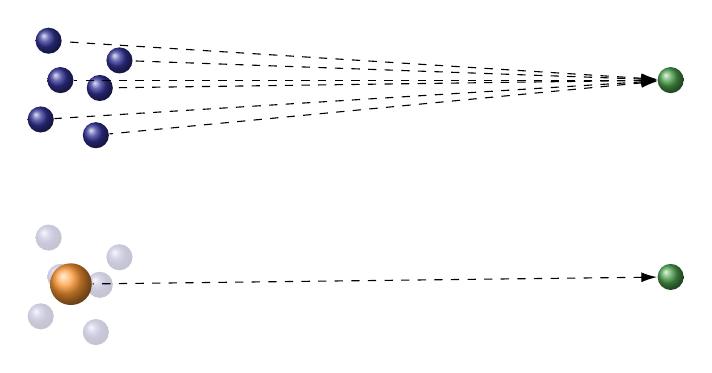
\begin{tikzpicture}
  \begin{scope}
      \node[shading=ball,circle,ball color=NavyBlue!80!white] at (0, 0) (m0) {};
      \node[shading=ball,circle,ball color=NavyBlue!80!white] at (1, 0.75) (m1) {};
      \node[shading=ball,circle,ball color=NavyBlue!80!white] at (.25, 0.5) (m2) {};
      \node[shading=ball,circle,ball color=NavyBlue!80!white] at (0.1, 1) (m3) {};
      \node[shading=ball,circle,ball color=NavyBlue!80!white] at (.75, .4) (m4) {};
      \node[shading=ball,circle,ball color=NavyBlue!80!white] at (.7, -.2) (m5) {};
      
      \node[shading=ball,circle,ball color=ForestGreen!80!white] at (8, .5) (mm) {};
      
      \foreach \x in {0,...,5}
        \draw[dashed, <-] (mm) edge (m\x);
  \end{scope}
  \begin{scope}[shift={(0, -2.5)}]
      \node[shading=ball,circle,ball color=NavyBlue!80!white,opacity=.25] at (0, 0) (m0) {};
      \node[shading=ball,circle,ball color=NavyBlue!80!white,opacity=.25] at (1, 0.75) (m1) {};
      \node[shading=ball,circle,ball color=NavyBlue!80!white,opacity=.25] at (.25, 0.5) (m2) {};
      \node[shading=ball,circle,ball color=NavyBlue!80!white,opacity=.25] at (0.1, 1) (m3) {};
      \node[shading=ball,circle,ball color=NavyBlue!80!white,opacity=.25] at (.75, .4) (m4) {};
      \node[shading=ball,circle,ball color=NavyBlue!80!white,opacity=.25] at (.7, -.2) (m5) {};
      
      \node[shading=ball,circle,scale=1.6,ball color=orange!80!white] at (.3833, .4083) (mcof) {};
  
      \node[shading=ball,circle,ball color=ForestGreen!80!white] at (8, .5) (mm) {};
      
      \draw[dashed, <-] (mm) edge (mcof);
  \end{scope}
  \begin{scope}[overlay]
    \draw[dotted, ->] (-.9, .4803) to [out=210,in=150] (-.9, .4803 + -2.5);
    \node[rotate=90] at (-1.8, .4803 + (-2.5 / 2) {\scriptsize approximation};
  \end{scope}
  \end{tikzpicture}
  \end{center}
  \vfill
  \setfontsize{8pt}
  See: \texttt{Josh Barnes and Piet Hut: A hierarchical O(N log N) force-calculation algorithm (1986)\\[-.5em]
  (DOI: \url{https://doi.org/10.1038/324446a0})}
\end{frame}
%%%%%%%%%%%%%%%%%%%%%%%%%%%%%%%%%%%%%%%%%%%%%%%%%%%%%%%%%%%%%%%%%%%%

%%%%%%%%%%%%%%%%%%%%%%%%%%%%%%%%%%%%%%%%%%%%%%%%%%%%%%%%%%%%%%%%%%%%
\begin{frame}[fragile]
  \frametitle{Theory: Barnes-Hut - Example: Quadtree}
  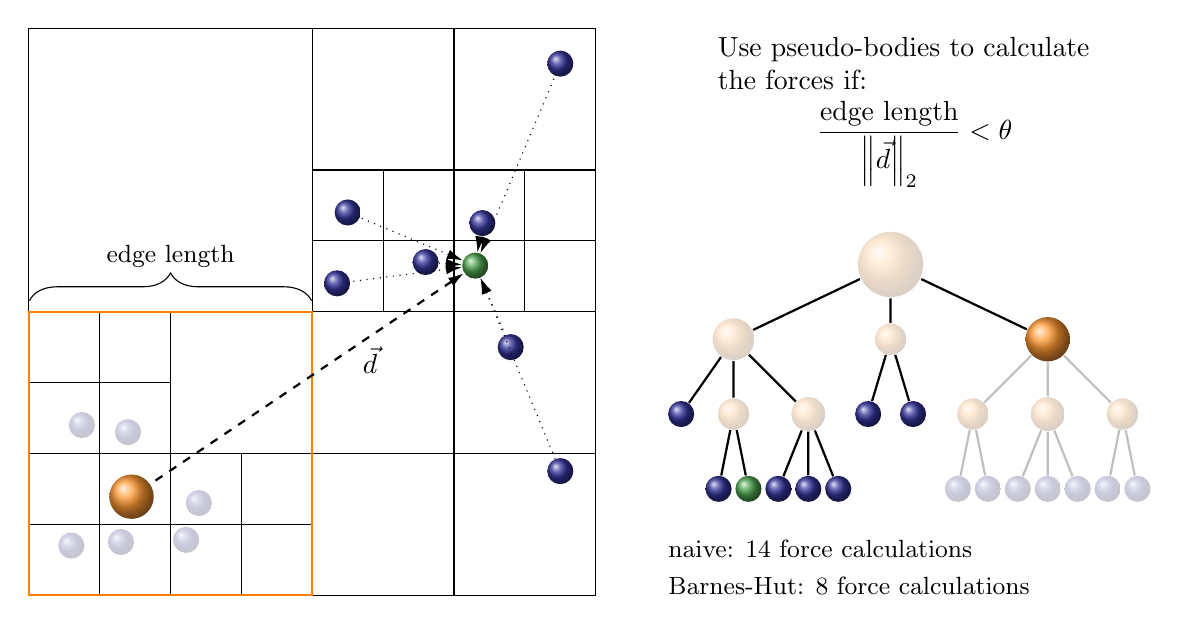
\begin{tikzpicture}
    \begin{scope}[scale=0.9]
        % Quadtree grid
        \draw[step=4] (0, 0) grid (8, 8);
        
        \draw[step=2] (0, 0) grid (4, 4);
        \draw[step=2] (4, 4) grid (8, 8);
        \draw[step=2] (4, 0) grid (8, 4);
        
        \draw[step=1] (0, 0) grid (2, 2);
        \draw[step=1] (0, 2) grid (2, 4);
        \draw[step=1] (2, 0) grid (4, 2);
        \draw[step=1] (4, 4) grid (6, 6);
        \draw[step=1] (6, 4) grid (8, 6);
        
        \draw[thick,orange] (0, 0) rectangle (4, 4);
        
        
        % bodies
        % top left
        
        % top right
        % 1.337
        \node[shading=ball,circle,ball color=NavyBlue!80!white] (p1) at (4.35, 4.4) {};
        \node[shading=ball,circle,ball color=NavyBlue!80!white] (p2) at (4.5, 5.4) {};
        \node[shading=ball,circle,ball color=NavyBlue!80!white] (p3) at (5.6, 4.7) {};
        
        \node[shading=ball,circle,ball color=ForestGreen!80!white] (p) at (6.3, 4.65) {};
        \node[shading=ball,circle,ball color=NavyBlue!80!white] (p4) at (6.4, 5.25) {};
        \node[shading=ball,circle,ball color=NavyBlue!80!white] (p5) at (7.5, 7.5) {};
        
        % bottom left
        \node[shading=ball,circle,ball color=NavyBlue!80!white,opacity=.25] at (1.5, 1.5) {};
        \node[shading=ball,circle,ball color=NavyBlue!80!white,opacity=.25] at (0.6, 0.7) {};
        \node[shading=ball,circle,ball color=NavyBlue!80!white,opacity=.25] at (1.4, 2.3) {};
        \node[shading=ball,circle,ball color=NavyBlue!80!white,opacity=.25] at (0.75, 2.4) {};
        \node[shading=ball,circle,ball color=NavyBlue!80!white,opacity=.25] at (1.3, 0.75) {};
        \node[shading=ball,circle,ball color=NavyBlue!80!white,opacity=.25] at (2.22, 0.78) {};
        \node[shading=ball,circle,ball color=NavyBlue!80!white,opacity=.25] at (2.4, 1.3) {};
        
        % center of mass of distant bodies
        \node[shading=ball,circle,scale=1.7,ball color=orange!80!white] (pp) at (1.45, 1.39) {}; % 0.6844
        
        % bottom right % 1.821
        \node[shading=ball,circle,ball color=NavyBlue!80!white] (p6) at (7.5, 1.75) {}; % 0.637
        \node[shading=ball,circle,ball color=NavyBlue!80!white] (p7) at (6.8, 3.5) {}; % 1.594
        
        
        % theta
        \draw[thick,dashed,<-] (p) -- (pp) node[midway, pos=.3, below] {$\vec{d}$};
        \draw [decorate,decoration={brace,amplitude=10pt,raise=4pt}] (0.01, 4) -- (3.99, 4) node [midway,yshift=.7cm] {\small edge length};
        \foreach \x in {1,...,7}
            \draw[dotted,<-] (p) -- (p\x);
    \end{scope}
    
    \begin{scope}[overlay, scale=0.9]
        \node[align=left,text width=5cm] (nt) at (12.5, 7.5) {Use pseudo-bodies to calculate the forces if:};
        \node[align=center, below=-.1cm of nt] {$\dfrac{\text{edge length}}{\norm{\vec{d}}_2} < \theta$};
    \end{scope}
    \begin{scope}[shift={(8, -1.5)}, scale=0.95]
        \node[shading=ball,circle,scale=2.5,ball color=orange!80!white,opacity=.25] (root) at (3.1, 6) {};
        
        % top right
        \node[shading=ball,circle,scale=1.6,ball color=orange!80!white,opacity=.25] (l11) at (1, 5) {};
        \node[shading=ball,circle,ball color=NavyBlue!80!white] (l21) at (0.3, 4) {};
        \node[shading=ball,circle,scale=1.2,ball color=orange!80!white,opacity=.25] (l22) at (1, 4) {};
        \node[shading=ball,circle,ball color=NavyBlue!80!white] (l31) at (0.8, 3) {};
        \node[shading=ball,circle,ball color=ForestGreen!80!white] (l32) at (1.2, 3) {};
        \node[shading=ball,circle,scale=1.3,ball color=orange!80!white,opacity=.25] (l23) at (2, 4) {};
        \node[shading=ball,circle,ball color=NavyBlue!80!white] (l33) at (1.6, 3) {};
        \node[shading=ball,circle,ball color=NavyBlue!80!white] (l34) at (2, 3) {};
        \node[shading=ball,circle,ball color=NavyBlue!80!white] (l35) at (2.4, 3) {};
        
        \draw[thick] (root) -- (l11);
        \draw[thick] (l11) -- (l21);
        \draw[thick] (l11) -- (l22);
        \draw[thick] (l11) -- (l23);
        \draw[thick] (l22) -- (l31);
        \draw[thick] (l22) -- (l32);
        \draw[thick] (l23) -- (l33);
        \draw[thick] (l23) -- (l34);
        \draw[thick] (l23) -- (l35);
        
        % bottom right
        \node[shading=ball,circle,scale=1.2,ball color=orange!80!white,opacity=.25] (l12) at (3.1, 5) {};
        \node[shading=ball,circle,ball color=NavyBlue!80!white] (l24) at (2.8, 4) {};
        \node[shading=ball,circle,ball color=NavyBlue!80!white] (l25) at (3.4, 4) {};
        \draw[thick] (root) -- (l12);
        \draw[thick] (l12) -- (l24);
        \draw[thick] (l12) -- (l25);
        
        % bottom left
        \node[shading=ball,circle,scale=1.7,ball color=orange!80!white] (l13) at (5.2, 5) {};
        \node[shading=ball,circle,scale=1.2,ball color=orange!80!white,opacity=.25] (l26) at (4.2, 4) {};
        \node[shading=ball,circle,ball color=NavyBlue!80!white,opacity=.25] (l36) at (4.4, 3) {};
        \node[shading=ball,circle,ball color=NavyBlue!80!white,opacity=.25] (l37) at (4, 3) {};
        \node[shading=ball,circle,scale=1.3,ball color=orange!80!white,opacity=.25] (l27) at (5.2, 4) {};
        \node[shading=ball,circle,ball color=NavyBlue!80!white,opacity=.25] (l38) at (4.8, 3) {};
        \node[shading=ball,circle,ball color=NavyBlue!80!white,opacity=.25] (l39) at (5.2, 3) {};
        \node[shading=ball,circle,ball color=NavyBlue!80!white,opacity=.25] (l310) at (5.6, 3) {};
        \node[shading=ball,circle,scale=1.2,ball color=orange!80!white,opacity=.25] (l28) at (6.2, 4) {};
        \node[shading=ball,circle,ball color=NavyBlue!80!white,opacity=.25] (l311) at (6, 3) {};
        \node[shading=ball,circle,ball color=NavyBlue!80!white,opacity=.25] (l312) at (6.4, 3) {};
        \draw[thick] (root) -- (l13);
        \draw[thick,opacity=.25] (l13) -- (l26);
        \draw[thick,opacity=.25] (l13) -- (l27);
        \draw[thick,opacity=.25] (l13) -- (l28);
        \draw[thick,opacity=.25] (l26) -- (l36);
        \draw[thick,opacity=.25] (l26) -- (l37);
        \draw[thick,opacity=.25] (l27) -- (l38);
        \draw[thick,opacity=.25] (l27) -- (l39);
        \draw[thick,opacity=.25] (l27) -- (l310);
        \draw[thick,opacity=.25] (l28) -- (l311);
        \draw[thick,opacity=.25] (l28) -- (l312);
        
        \node[anchor=west] at (0, 2.2) {\small naive: $\num{14}$ force calculations};
        \node[anchor=west] at (0, 1.7) {\small Barnes-Hut: $\num{8}$ force calculations};
    \end{scope}
  \end{tikzpicture}
\end{frame}
%%%%%%%%%%%%%%%%%%%%%%%%%%%%%%%%%%%%%%%%%%%%%%%%%%%%%%%%%%%%%%%%%%%%

%%%%%%%%%%%%%%%%%%%%%%%%%%%%%%%%%%%%%%%%%%%%%%%%%%%%%%%%%%%%%%%%%%%%
\begin{frame}[fragile]
  \frametitle{Theory: Barnes-Hut - Tree Node}
  Each node of the octree (extension of the quadtree for the $3$-dimensional space) has to save the following information:
  \begin{itemize}
      \item edge length of the octree-octant
      \item sum of the masses of all bodies in the octant: $m_{oct} = \sum_i m_i$
      \item center of mass of all bodies $i$ in the octant: $\vec{c}_{oct} = \dfrac{\sum_i m_i \vec{r}_i}{\sum_i m_i}$
      \item all children of the octant
  \end{itemize}
  \vfill
  Each leaf may only contain a single body!
\end{frame}
%%%%%%%%%%%%%%%%%%%%%%%%%%%%%%%%%%%%%%%%%%%%%%%%%%%%%%%%%%%%%%%%%%%%

%%%%%%%%%%%%%%%%%%%%%%%%%%%%%%%%%%%%%%%%%%%%%%%%%%%%%%%%%%%%%%%%%%%%
\begin{frame}[fragile]
  \frametitle{Theory: Barnes-Hut - Update the Accelerations $\vec{a}_i$}
  \begin{algorithmcl}
    \begin{algorithmic}[1]
        \Procedure{UpdateAcceleration}{\texttt{body}, \texttt{node}}
        \State{calculate direction vector $\vec{d}$ between \texttt{body} and the center of mass of \texttt{node}}
        \If{pseudo-body can be used $\vee$ \texttt{node} is leaf}
            \State{update acceleration of $\vec{a}_\text{\texttt{body}}$}
        \Else
            \For{each \texttt{child} of \texttt{node}}
                \State{\textsc{UpdateAcceleration}(\texttt{body}, \texttt{child})}
            \EndFor
        \EndIf
        \EndProcedure
    \end{algorithmic}
  \end{algorithmcl}
  \vfill
  \textbf{Question:}\\
  Is it also possible to speed up the force calculations using the Barnes-Hut tree?
\end{frame}
%%%%%%%%%%%%%%%%%%%%%%%%%%%%%%%%%%%%%%%%%%%%%%%%%%%%%%%%%%%%%%%%%%%%

\subsection{Time Stepping Method}
%%%%%%%%%%%%%%%%%%%%%%%%%%%%%%%%%%%%%%%%%%%%%%%%%%%%%%%%%%%%%%%%%%%%
\begin{frame}[fragile]
  \frametitle{Theory: Leapfrog Integration}
  The leapfrog integration, a 2nd order time step method, as a combination of the two variants of the symplectic Euler method (SE), is used to advance from the time step $k$ to the next time step $k + 1$:
  \begin{equation*}
    \begin{split}
      (SE1) &\left\lbrace
      \begin{array}{rcl}
        \vec{v}^{k+\frac{1}{2}} & = & \vec{v}^k + \vec{a}^k \frac{\Delta t}{2}               \\
        \vec{r}^{k+\frac{1}{2}} & = & \vec{r}^k + \vec{v}^{k + \frac{1}{2}} \frac{\Delta t}{2}
      \end{array}\right.\\[.5em]
      (SE2) &\left\lbrace
      \begin{array}{rcl}
        \vec{r}^{k+1} & = & \vec{r}^{k + \frac{1}{2}} + \vec{v}^{k + \frac{1}{2}} \frac{\Delta t}{2} \\
        \vec{v}^{k+1} & = & \vec{v}^{k + \frac{1}{2}} + \vec{a}^{k+1} \frac{\Delta t}{2}
      \end{array}\right.\\
    \end{split}
  \end{equation*} \\
  \vfill
  \setfontsize{8pt}
  See: \texttt{O. Buneman: Time-Reversible Difference Procedures (1967)\\[-.5em]
  (DOI: \url{https://doi.org/10.1016/0021-9991(67)90056-3})}
  % https://www.sciencedirect.com/science/article/pii/0021999167900563
  % https://www.sciencedirect.com/science/article/pii/0010465587900191
\end{frame}
%%%%%%%%%%%%%%%%%%%%%%%%%%%%%%%%%%%%%%%%%%%%%%%%%%%%%%%%%%%%%%%%%%%%

\subsection{Complete Simulation}
%%%%%%%%%%%%%%%%%%%%%%%%%%%%%%%%%%%%%%%%%%%%%%%%%%%%%%%%%%%%%%%%%%%%
\begin{frame}<1>[fragile, label={complete_simulation}]
  \frametitle<1>{Theory: A Complete Simulation}
  \frametitle<2>{A Complete Simulation}
\begin{algorithmcl}
    \begin{algorithmic}[1]
        \State{adjust initial velocities: $\vec{u}_i = \dfrac{\sum_j m_j \vec{v}_j}{\sum_j m_j}$;\quad$\vec{v}_i = \vec{v}_i - \vec{u}_i$}
        \State{update accelerations $\vec{a}_i$}
        \State{visualize initial state}
        \While{simulation not terminated yet}
            \State{perform leapfrog integration step}
            \If{time step should be visualized}
                \State{visualize time step}
            \EndIf
            \State{update time step}
        \EndWhile
        \State{Save final state of the simulation as \texttt{.csv} file (name + mass + positions + velocities)}
    \end{algorithmic}
\end{algorithmcl}
    \only<2>{\vfill\textbf{Question:} What can and should be parallelized?}
\end{frame}
%%%%%%%%%%%%%%%%%%%%%%%%%%%%%%%%%%%%%%%%%%%%%%%%%%%%%%%%%%%%%%%%%%%%

\section{Simulation Data}
%%%%%%%%%%%%%%%%%%%%%%%%%%%%%%%%%%%%%%%%%%%%%%%%%%%%%%%%%%%%%%%%%%%%
\begin{frame}
    \frametitle{The Simulation Data}
    Two data sets given in \link{\urlIliasData}{ILIAS}:
    \begin{itemize}
        \item Planets, dwarf planets, and (named) moons (feel free to add the data of the remaining moons if you can find them and let us know!) in our solar system. \\[.25em]
        \itFollows{This data can be used for development, debugging, and verification.}
        \item The asteroid data used in scenario 1.
    \end{itemize}
    \pause
    \vfill
    More asteroid data for scenario 2 can be downloaded using NASA Jet Propulsion Laboratory's (JPL) \link{https://ssd.jpl.nasa.gov/tools/sbdb_query.html}{Small-Body Database}:%
    \begin{itemize}
        \item select desired orbit class(es)
        \item add orbit constraints: e.g., \texttt{albedo} and \texttt{diameter} must be defined (Physical Parameter Fields)
        \item select necessary Fields (for the name use the \texttt{IAU name} field)
    \end{itemize}
    This allows you to generate nearly arbitrarily large data sets using real-world data: $\approx\num{140000}$ asteroids with defined \texttt{albedo} and \texttt{diameter} and over one million asteroids in total.
\end{frame}
%%%%%%%%%%%%%%%%%%%%%%%%%%%%%%%%%%%%%%%%%%%%%%%%%%%%%%%%%%%%%%%%%%%%

%%%%%%%%%%%%%%%%%%%%%%%%%%%%%%%%%%%%%%%%%%%%%%%%%%%%%%%%%%%%%%%%%%%%
\begin{frame}[fragile]
    \frametitle{The Simulation Data - Format}

    You need to be able to parse the following \texttt{.csv} file:
    \begin{minted}[breaklines, fontsize=\scriptsize]{text}
e,a,i,om,w,ma,epoch,H,albedo,diameter,class,name,mass,central_body
0.2056302515978038,0.3870982252718477,7.005014362233553,48.33053877672862,29.12427943500334, 172.7497133441682,2451544.5,,,,PLA,Mercury,3.301011e+23,Sun
.2227328427416296,1.4581505451557,10.82795835269297,304.2910556026917,178.9325148860407, 358.8212586092838,2459800.5,10.31,0.25,16.84,AMO,Eros,,
    \end{minted}
    \vfill
    \mintinline{text}{e,a,i,om,w,ma,epoch}: as part of the Keplerian orbital elements. \\
    \mintinline{text}{H,albedo,diameter,mass}: to estimate the mass of a body if not given. \\
    \mintinline{text}{class}: the orbital class of the body. \\
    \mintinline{text}{name}: the \link{https://en.wikipedia.org/wiki/Astronomical_naming_conventions}{IAU name} of the body. \\
    \mintinline{text}{central_body}: the name of the central body.
\end{frame}
%%%%%%%%%%%%%%%%%%%%%%%%%%%%%%%%%%%%%%%%%%%%%%%%%%%%%%%%%%%%%%%%%%%%

%%%%%%%%%%%%%%%%%%%%%%%%%%%%%%%%%%%%%%%%%%%%%%%%%%%%%%%%%%%%%%%%%%%%
\begin{frame}
    \frametitle{The Simulation Data - General Remarks}
    \begin{itemize}
        \item Independent of the used JPL asteroid data set, the planets and moon data set must \textbf{always} be included in your simulation!
        \item Be aware that the angles are given in degrees and not in radians.
        \item Be aware that some bodies may appear multiple times (e.g., Pluto and its moons) and you have to ensure that these bodies are only used once in the actual simulation!
        \item All data must be saved and processed using double precision (FP64, \mintinline{c++}{double}) floating point types.
        \item \textbf{Attention:} The Sun/Sol (with the reference mass \SI{1.98847e30}{\kilo\gram} and epoch $2451544.5$ JD) must always be \textbf{manually} added at the coordinate's origin since it is impossible to specify its orbital elements with respect to itself.
    \end{itemize}
\end{frame}
%%%%%%%%%%%%%%%%%%%%%%%%%%%%%%%%%%%%%%%%%%%%%%%%%%%%%%%%%%%%%%%%%%%%
\section{Value Approximation}
%%%%%%%%%%%%%%%%%%%%%%%%%%%%%%%%%%%%%%%%%%%%%%%%%%%%%%%%%%%%%%%%%%%%
\begin{frame}
    \frametitle{Value Approximation}
    
    Some values or columns may not be present and, therefore, must be approximated:
    \begin{itemize}
        \item the \texttt{mass} column does not exist in the JPL data sets: it must be estimated using the asteroid's \texttt{diameter} and geometric \texttt{albedo}.
        \item If no \texttt{albedo} is given, approximate it using the asteroid's orbit class.
        \item If no \texttt{diameter} is given, approximate it using the asteroid's absolute magnitude \texttt{H} and geometric \texttt{albedo}.
        \item The \texttt{central\_body} column does not exist in the JPL data sets: by definition, the \texttt{central\_body} of all asteroids is the Sun/Sol.
    \end{itemize}
\end{frame}


%%%%%%%%%%%%%%%%%%%%%%%%%%%%%%%%%%%%%%%%%%%%%%%%%%%%%%%%%%%%%%%%%%%%
\begin{frame}[label={orbit_classes}]
    \frametitle{Value Approximation - Geometric Albedo}
    \btVFill
    Approximate the assumed geometric \texttt{albedo} using random number distributions based on the asteroid's orbit class:
    \begin{columns}
        \begin{column}{.5\linewidth}
            \setfontsize{9pt}
            \begin{description}
                \item[AMO] (Amor): $\interval{0.450}{0.550}$
                \item[APO] (Apollo): $\interval{0.450}{0.550}$
                \item[ATE] (Aten): $\interval{0.450}{0.550}$
                \item[IEO] (Interior Earth Obj.): $\interval{0.450}{0.550}$
                \item[MCA] (Mars-crossing): $\interval{0.450}{0.550}$
                \item[IMB] (Inner Main-belt): $\interval{0.030}{0.103}$
                \item[MBA] (Main-belt): $\interval{0.097}{0.203}$
            \end{description}   
        \end{column}
        \hspace*{-1cm}
        \begin{column}{.55\linewidth}
            \setfontsize{9pt}
            \begin{description}
                \item[OMB] (Outer Main-belt): $\interval{0.197}{0.5}$
                \item[CEN] (Centaur): $\interval{0.450}{0.750}$
                \item[TJN] (Jupiter Trojans): $\interval{0.188}{0.124}$
                \item[TNO] (TransNeptunian Obj.): $\interval{0.022}{0.130}$
                \item[AST] (Asteroid): $\interval{0.450}{0.550}$
                \item[PAA] (Parabolic): $\interval{0.450}{0.550}$
                \item[HYA] (Hyperbolic): $\interval{0.450}{0.550}$
            \end{description}
        \end{column}
    \end{columns}
    \vspace*{.5em}
    \textbf{Note:} These are just very rough estimates, if you find more accurate estimates feel free to use them and let us know!
    \btVFill
    \visible<2->{
        We also added four new orbit classes (for a better ParaView output):
        \begin{columns}
            \begin{column}{.5\linewidth}
                \setfontsize{9pt}
                \begin{description}
                    \item[STA] (Star): the Sun/Sol
                    \item[PLA] (Planets): Earth, Mars, $\dots$
                \end{description}   
            \end{column}
            \hspace*{-1cm}
            \begin{column}{.55\linewidth}
                \setfontsize{9pt}
                \begin{description}
                    \item[DWA] (Dwarf Planets): Ceres, Pluto, Eris, $\dots$
                    \item[SAT] (Satellites (Moons)): Luna, Titan, $\dots$
                \end{description}
            \end{column}
        \end{columns}
    }
    \btVFill
    \setfontsize{8pt}
    See: \url{https://pdssbn.astro.umd.edu/data_other/objclass.shtml}
\end{frame}
%%%%%%%%%%%%%%%%%%%%%%%%%%%%%%%%%%%%%%%%%%%%%%%%%%%%%%%%%%%%%%%%%%%%

%%%%%%%%%%%%%%%%%%%%%%%%%%%%%%%%%%%%%%%%%%%%%%%%%%%%%%%%%%%%%%%%%%%%
\begin{frame}
    \frametitle{Value Approximation - Diameter}
    \btVFill
    Approximate the diameter $d$ of an asteroid given its assumed geometric \texttt{albedo} and absolute magnitude $H$ using:
    \begin{flalign*}
        &&& d = 1329 \cdot \texttt{albedo}^{-0.5} \cdot 10^{-0.2H}
        && [\si{\kilo\meter}]
    \end{flalign*}
    \btVFill
    \setfontsize{8pt}
    See: \texttt{B. Carry: Density of asteroids (2012)\\[-.2em]
    (DOI: \url{https://doi.org/10.1016/j.pss.2012.03.009})}
\end{frame}

%%%%%%%%%%%%%%%%%%%%%%%%%%%%%%%%%%%%%%%%%%%%%%%%%%%%%%%%%%%%%%%%%%%%
\begin{frame}
    \frametitle{Value Approximation - Mass}
    Approximate the density $\rho$ of an asteroid given its assumed geometric \texttt{albedo} based on the three main asteroid categories: 
    \begin{description}
        \item[C-type] (chondrite): most common, probably consist of clay and silicate rocks; \\
        assumption: $\texttt{albedo} < \num{0.1} \quad\rightarrow\quad \rho = \SI{1.38}{\gram\per\cm^3}$ 
        \item[S-type] (\enquote{stony}): made up of silicate materials and nickel-iron;\\
        assumption: $\num{0.1} \leq \texttt{albedo} \leq \num{0.2} \quad\rightarrow\quad \rho = \SI{2.71}{\gram\per\cm^3}$ 
        \item[M-type] (nickel-iron): metallic;\\
        assumption: $\texttt{albedo} > \num{0.2} \quad\rightarrow\quad \rho = \SI{5.32}{\gram\per\cm^3}$ 
    \end{description}
    \vfill
    \visible<2->{
        Approximate the mass of the asteroid using its presumed density $\rho$ and its diameter $d$ assuming a spherical shape via (\textbf{note:} pay attention to the physical units!):
        
        \begin{flalign*}
            &&& m = \dfrac{4}{3}\pi \cdot \left(\dfrac{d}{2}\right)^3 \cdot \rho
            && [\si{\kilo\gram}]
        \end{flalign*}
    }
    \btVFill
    \setfontsize{8pt}
    See: \url{https://solarsystem.nasa.gov/asteroids-comets-and-meteors/asteroids/in-depth/}
\end{frame}
%%%%%%%%%%%%%%%%%%%%%%%%%%%%%%%%%%%%%%%%%%%%%%%%%%%%%%%%%%%%%%%%%%%%
\section{Keplerian Orbital Elements}
%%%%%%%%%%%%%%%%%%%%%%%%%%%%%%%%%%%%%%%%%%%%%%%%%%%%%%%%%%%%%%%%%%%%
\begin{frame}
    \frametitle{Phase 1.3: Orbital Elements to Orbital State Vectors}
    \begin{itemize}
        \item For our n-body simulation, we need the two Cartesian vectors for each body: the position vector $\vec{r}$ and the velocity vector $\vec{v}$. 
        \item They are also called \textit{orbital state vectors}.
        \vspace*{1em}
        \item In astronomy the Kepler orbit is used more often to describe the mechanics of a celestial body.
        \item They are also called Keplerian \textit{orbital elements}.
    \end{itemize}
    \pause
    \vfill
    \itFollows{Since the data is given using the orbital elements, we must convert them to their respective orbital state vectors before we can use them in our simulation.}
\end{frame}
%%%%%%%%%%%%%%%%%%%%%%%%%%%%%%%%%%%%%%%%%%%%%%%%%%%%%%%%%%%%%%%%%%%%

\subsection{Definition}
%%%%%%%%%%%%%%%%%%%%%%%%%%%%%%%%%%%%%%%%%%%%%%%%%%%%%%%%%%%%%%%%%%%%
\begin{frame}
    \frametitle{Orbital Elements - Visualization: Shape and Size of the Ellipsis}
    \begin{center}
        \begin{tikzpicture}
\begin{scope}
    \shade[ball color = gray!40, opacity = 0.8] (0,0) circle (.2cm);
    \visible<2->{
        \draw (0, 0) circle (2cm);
        \node at (0, -2.5) {$e = 0$};
    };
    \visible<3->{
        \draw[dashed] (-2, 0) -- (0, 0);
        \draw[dashed] (0, 2) -- (0, -2);
        \draw[red] (0, 0) -- node[below=5pt] {$a$} ++(2, 0);
        \fill (0, 0) circle (.05cm);
    };
\end{scope}
\begin{scope}[shift={(6,0)}]
    \shade[ball color = gray!40, opacity = 0.8] (-.25,0) circle (.2cm);
    \visible<2->{
        \draw (1, 0) ellipse (2cm and 1.5cm);
        \node at (1, -2.5) {$e = \num{0.66}$};
    };
    \visible<3->{
        \draw[dashed] (-1, 0) -- (1, 0);
        \draw[dashed] (1, 1.5) -- (1, -1.5);
        \draw[red] (1, 0) -- node[below=5pt] {$a$} ++(2, 0);
        \fill (1, 0) circle (.05cm);
    };
\end{scope}
        \end{tikzpicture}
    \end{center}
    \begin{description}
        \setlength\itemsep{.5em}
        \item<2->[eccentricity $e$]\hfill\\\hspace*{-2cm} shape of the ellipsis (elongation compared to a circle)
        \item<3->[{semi-major axis $a\ [\si{\au}]$}]\hfill\\\hspace*{-2cm} one-half of the largest diameter
    \end{description}
\end{frame}
%%%%%%%%%%%%%%%%%%%%%%%%%%%%%%%%%%%%%%%%%%%%%%%%%%%%%%%%%%%%%%%%%%%%

%%%%%%%%%%%%%%%%%%%%%%%%%%%%%%%%%%%%%%%%%%%%%%%%%%%%%%%%%%%%%%%%%%%%
\begin{frame}[t]
    \frametitle{Orbital Elements - Visualization}
    \vspace*{-.9em}
    \begin{center}
        \begin{tikzpicture}[scale=1.1]
% reference plane
\draw[fill, color=gray!20] (-4, -1.5) -- (5.8, -1.5) -- (5, 1.5) -- (-4.8, 1.5) -- cycle;

% reference direction
\draw[color=gray!90, ->] (0, 0) -- (4, 0);
\node at (4.2, -.2) {\Aries};

\visible<6-|handout:6>{
    % argument of periapsis
    \draw[dashed, ForestGreen] (0, 0) -- (2.98, 1.98);
    \node (ap1) at (.12, -.4) {};
    \node (ap2) at (.925, .6) {};
    \draw[thick, ForestGreen, ->] (ap1.center) to[bend right=40, in=260] (ap2.center);
    \node[ForestGreen] at (.8, .25) {$\omega$};
}

\visible<7-|handout:7->{
    % true/mean anomaly
    \draw[dashed, red] (0, 0) -- (1.8, 2.2);
    \node (tma1) at (1.875, 1.25) {};
    \node (tma2) at (1.25, 1.525) {};
    \draw[thick, red, ->] (tma1.center) to[bend right=40, out=310] (tma2.center);
    \node[red] at (1.45, 1.275) {$\nu$};
}

\visible<2-|handout:2->{
    % orbit
    \draw[thick, rotate=30, opacity=0.75] (0.0, 0.0) ellipse (3.61cm and 1.5cm);
    \fill[color=gray!20, opacity=0.75] (-.35, 1.5) rectangle (-4, -1.5);
    \fill[white, opacity=0.6] (-4, -1.5) rectangle (.4, -2.5);
    % orbital body
    \shade[ball color=red!40] (1.8, 2.2) circle (.15cm);
    \node (obd1) at (1.8 + .45, 2.35) {};
    \node (obd2) at (1.8 - .45, 2.25) {};
    \draw[->] (obd1) to[bend right=20] (obd2);
}

\visible<3-|handout:3->{
    % inclination
    \node (i1) at (1.4, -1.5) {};
    \node (i2) at (1.3, -0.95) {};
    \draw[thick, blue, ->] (i1.center) to[bend right=40] (i2.center);
    \node[blue] (i) at (1.15, -1.275) {\bfseries $i$};
}

\visible<4-|handout:4->{
    % ascending node 
    \draw[dotted, color=gray!40] (.4, -1.5) -- (-.4, 1.5);
    \fill (.4, -1.5) circle (.05cm);
    \node at (.4, -1.85) {
\includegraphics[width=.3cm]{figures/ascending_node}};
}
\visible<5-|handout:5->{
    % longitude of the ascending node
    \node (lan1) at (.6, 0) {};
    \node (lan2) at (.1, -.6) {};
    \draw[thick, orange, ->] (.45, 0) arc[start angle=0, end angle=280, x radius=.45, y radius=.25];
    \node[orange] at (-.7, 0) {$\Omega$};
}

% central body
\shade[ball color=gray!40] (0, 0) circle (.2cm);
\draw[fill, color=gray!20, opacity=0.75] (-0.2, -0.01) rectangle (0.2, -0.2);
        \end{tikzpicture}
    \end{center}
    \vspace*{.15em}
    
    \begin{tikzpicture}[overlay]
\only<1|handout:1>{
    \node[minimum size=\textwidth, align=left, anchor=west] at (-2.4, 0) {%
    reference direction \Aries:\\
    for heliocentric orbits also known as \enquote{First Point of Aries}};
}
\only<3|handout:3>{
    \node[minimum size=\textwidth, align=left, anchor=west] at (-.3, 0) {%
    \begin{varwidth}{\linewidth}
        \begin{description}
            \item[{inclination $i\ [\si{rad}]$}]\hfill\\\hspace*{-2cm} 
            vertical tilt of the ellipsis with respect to the reference plane, e.g.:\\\hspace*{-1cm}
            \begin{tabular}{r@{\hspace{3pt}}c@{\hspace{3pt}}rl}
                $\SI{0}{\radian}$ & $=$ & $\SI{0}{\degree}$ & orbital plane same as reference plane \\
                $\SI{1.5708}{\radian}$ & $=$ & $\SI{90}{\degree}$ & orbital plane perpendicular to reference plane
            \end{tabular}
        \end{description}
    \end{varwidth}};
}
\only<4|handout:4>{
    \node[minimum size=\textwidth, align=left, anchor=west] at (-1.3, 0) {%
    ascending node 
\includegraphics[width=.3cm]{figures/ascending_node}:\\
    point where the orbiting body moves \textbf{north} through the reference plane};
}
\only<5|handout:5>{
    \node[minimum size=\textwidth, align=left, anchor=west] at (-.2, 0) {%
    \begin{varwidth}{\linewidth}
        \begin{description}
            \item[{longitude of the ascending node $\Omega\ [\si{\radian}]$}]\hfill\\\hspace*{-2cm}%
            the angle from the reference direction to the direction of the ascending node; \\\hspace*{-2cm}measured counterclockwise
        \end{description}
    \end{varwidth}};
}
\only<6|handout:6>{
    \node[minimum size=\textwidth, align=left, anchor=west] at (-.2, 0) {%
    \begin{varwidth}{\linewidth}
        \begin{description}
            \item[{argument of periapsis $\omega\ [\si{\radian}]$}]\hfill\\\hspace*{-2cm} 
            angle from the body's ascending node to its periapsis in the direction of motion, e.g.:\\\hspace*{-1cm}
            \begin{tabularx}{.9\textwidth}{rX}
                $\SI{0}{\radian}$ & the orbiting body has its closest approach to the central body at the same moment it crosses the reference frame from south to north 
            \end{tabularx}
        \end{description}
    \end{varwidth}};
}
\only<7|handout:7>{
    \node[minimum size=\textwidth, align=left, anchor=west] at (-.2, 0) {%
    true anomaly $\nu\ [\si{\radian}]$ at epoch $t_0\ [\si{\jd}]$:\\
    angle between the direction of periapsis and the position of the orbiting body at epoch $t_0$};
}
\only<8|handout:8>{
    \node[minimum size=\textwidth, align=left, anchor=west] at (-.2, 0) {%
    \begin{varwidth}{\linewidth}
        \begin{description}
            \item[{mean anomaly $M_0\ [\si{\radian}]$ at epoch $t_0\ [\si{\jd}]$}]\hfill\\\hspace*{-2cm} 
            the angular distance from the pericenter which a fictitious body would have if it \\\hspace*{-2cm}
            moved in a circular orbit, with constant speed, in the same orbital period as the \\\hspace*{-2cm}
            actual body in its elliptical orbit
        \end{description}
    \end{varwidth}};
}
    \end{tikzpicture}
\end{frame}
%%%%%%%%%%%%%%%%%%%%%%%%%%%%%%%%%%%%%%%%%%%%%%%%%%%%%%%%%%%%%%%%%%%%

%%%%%%%%%%%%%%%%%%%%%%%%%%%%%%%%%%%%%%%%%%%%%%%%%%%%%%%%%%%%%%%%%%%%
\begin{frame}
    \frametitle{Orbital Elements - The Six Keplerian Elements (Overview)}
    \hspace{0em}
    \vspace{-1.3em}
    \begin{description}
        \setlength\itemsep{.3em}
        \item[eccentricity $e$]\hfill\\\hspace*{-2cm} 
        shape of the ellipsis (elongation compared to a circle)
        \item[{semi-major axis $a\ [\si{\au}]$}]\hfill\\\hspace*{-2cm} 
        one-half of the largest diameter
        \item[{inclination $i\ [\si{\radian}]$}]\hfill\\\hspace*{-2cm} 
        vertical tilt of the ellipsis with respect to the reference plane
        \item[{longitude of the ascending node $\Omega\ [\si{\radian}]$}]\hfill\\\hspace*{-2cm} 
        the angle from the reference direction to the direction of the ascending node
        \item[{argument of periapsis $\omega\ [\si{\radian}]$}]\hfill\\\hspace*{-2cm}
        angle from the body's ascending node to its periapsis in the direction of motion
        \item[{mean anomaly $M_0\ [\si{\radian}]$ at epoch $t_0\ [\si{\jd}]$}]\hfill\\\hspace*{-2cm} the angular distance from the pericenter which a fictitious body would have if it \\\hspace*{-2cm}
        moved in a circular orbit, with constant speed, in the same orbital period as the \\\hspace*{-2cm}
        actual body in its elliptical orbit
    \end{description}
\end{frame}
%%%%%%%%%%%%%%%%%%%%%%%%%%%%%%%%%%%%%%%%%%%%%%%%%%%%%%%%%%%%%%%%%%%%

%%%%%%%%%%%%%%%%%%%%%%%%%%%%%%%%%%%%%%%%%%%%%%%%%%%%%%%%%%%%%%%%%%%%
\begin{frame}
    \frametitle{Orbital State Vectors - Cartesian Vectors}
    \begin{description}
        \setlength\itemsep{.5em}
        \item[{position $\vec{r}\ [\si{\au}]$}]\hfill\\\hspace*{-2cm} the position of the body in the reference frame, $\vec{r} \in \mathbb{R}^3$
        \item[{velocity $\vec{v}\ [\si{\au\per\day}]$}]\hfill\\\hspace*{-2cm} the velocity of the body in the same reference frame, $\vec{v} \in \mathbb{R}^3$
    \end{description}
\end{frame}
%%%%%%%%%%%%%%%%%%%%%%%%%%%%%%%%%%%%%%%%%%%%%%%%%%%%%%%%%%%%%%%%%%%%

\subsection{Conversion to state vectors}
%%%%%%%%%%%%%%%%%%%%%%%%%%%%%%%%%%%%%%%%%%%%%%%%%%%%%%%%%%%%%%%%%%%%
\begin{frame}
    \frametitle{Convert Orbital Elements to Orbital State Vectors - 1}
    \btVFill
    \begin{enumerate}
        \item Calculate $M(t)$:
        $$ M(t) = M_0 + (t - t_0) \sqrt{\frac{\mu}{a^3}} $$
        where $\mu = GM$ is the standard gravitational parameter of the central body and $t$ the Sun's/Sol's reference epoch at $2451544.5$ JD (midnight on January 1, 2000)\\
        (\textbf{note:} take care of the correct units!).
        \item Solve \textsc{Kepler}'s equation $M(t) = E(t) - e \sin{E(t)}$ for the eccentric anomaly $E(t)$ with a numerical method like \textsc{Newton-Raphson}:
        $$ E_0(t) = M(t) $$
        $$ E_{j+1}(t) = E_j(t) - \frac{E_j(t) - e \sin{E_j(t)} - M(t)}{1 - e \cos{E_j(t)}} $$
        using a suitable stopping criterion (e.g., a fixed number of \num{30} iterations).
    \end{enumerate}
    \btVFill
    \setfontsize{8pt}
    See: \url{https://downloads.rene-schwarz.com/download/M001-Keplerian_Orbit_Elements_to_Cartesian_State_Vectors.pdf}
\end{frame}
%%%%%%%%%%%%%%%%%%%%%%%%%%%%%%%%%%%%%%%%%%%%%%%%%%%%%%%%%%%%%%%%%%%%

%%%%%%%%%%%%%%%%%%%%%%%%%%%%%%%%%%%%%%%%%%%%%%%%%%%%%%%%%%%%%%%%%%%%
\begin{frame}
    \frametitle{Convert Orbital Elements to Orbital State Vectors - 2}
    \btVFill
    \begin{enumerate}
        \setcounter{enumi}{2}
        \item Calculate the true anomaly $\nu(t)$:
        $$ \nu(t) = 2 \cdot\arctan2\left(\sqrt{1 + e} \sin{\frac{E(t)}{2}}, \sqrt{1 - e} \cos{\frac{E(t)}{2}} \right) $$
        \item Calculate the distance to the central body:
        $$ r_c(t) = a(1 - e \cos{E(t)}) $$
        \item Calculate the position $\vec{o}(t)$ and velocity $\dot{\vec{o}}(t)$ vectors in the orbital frame:
        $$ \vec{o}(t) = r_c(t) \begin{pmatrix} \cos{\nu(t)} \\ \sin{\nu(t)} \\ 0 \end{pmatrix}, \quad
           \dot{\vec{o}}(t) = \frac{\sqrt{\mu a}}{r_c(t)} \begin{pmatrix} -\sin{E(t)} \\ \sqrt{1 - e^2} \cos{E(t)} \\ 0 \end{pmatrix} $$
    \end{enumerate}
    \btVFill
    \setfontsize{8pt}
    See: \url{https://downloads.rene-schwarz.com/download/M001-Keplerian_Orbit_Elements_to_Cartesian_State_Vectors.pdf}
\end{frame}
%%%%%%%%%%%%%%%%%%%%%%%%%%%%%%%%%%%%%%%%%%%%%%%%%%%%%%%%%%%%%%%%%%%%

%%%%%%%%%%%%%%%%%%%%%%%%%%%%%%%%%%%%%%%%%%%%%%%%%%%%%%%%%%%%%%%%%%%%
\begin{frame}
    \frametitle{Convert Orbital Elements to Orbital State Vectors - 3}
    \btVFill
    \begin{enumerate}
        \setcounter{enumi}{5}
        \item Transform $\vec{o}(t)$ and $\dot{\vec{o}}(t)$ to the inertial frame in bodycentric rectangular coordinates $\vec{r}(t)$ and $\dot{\vec{r}}(t)$ using the matrix $R$:
        $$R = \begin{pmatrix} 
                \cos{\omega}\cos{\Omega} - \sin{\omega}\cos{i}\sin{\Omega} & -(\sin{\omega}\cos{\Omega} + \cos{\omega}\cos{i}\sin{\Omega}) & 0 \\ 
                \cos{\omega}\sin{\Omega} + \sin{\omega}\cos{i}\cos{\Omega} & \cos{\omega}\cos{i}\cos{\Omega} - \sin{\omega}\sin{\Omega} & 0 \\ 
                \sin{\omega}\sin{i} & \cos{\omega}\sin{i} & 0
              \end{pmatrix}$$
        $$ \vec{r}(t) = R \cdot \vec{o}(t), \quad 
           \dot{\vec{r}}(t) = R \cdot \dot{\vec{o}}(t)$$
        % \item Convert $\vec{r}(t)$ and $\dot{\vec{r}}(t)$ to the respective output units $\si{\au}$ and $\si{\au\per\day}$:
        % $$ \vec{r}(t)_{[\si{\au}]} = \vec{r}(t) \cdot \frac{\num{1}}{\num{1.49597870691e11}}, $$
        % $$ \dot{\vec{r}}(t)_{[\si{\au\per\day}]} = \dot{\vec{r}}(t) \cdot \frac{\num{86400}}{\num{1.49597870691e11}} $$
        \item Update position and velocity to be relative to its central body $cb$:
        $$ \vec{r}(t) = \vec{r}(t) + \vec{r}_{cb}(t), \quad
           \dot{\vec{r}}(t) = \dot{\vec{r}}(t) + \dot{\vec{r}}_{cb}(t)$$
    \end{enumerate}
    \btVFill
    \setfontsize{8pt}
    See: \url{https://downloads.rene-schwarz.com/download/M001-Keplerian_Orbit_Elements_to_Cartesian_State_Vectors.pdf}
\end{frame}
%%%%%%%%%%%%%%%%%%%%%%%%%%%%%%%%%%%%%%%%%%%%%%%%%%%%%%%%%%%%%%%%%%%%
\section{Parallelization}
%%%%%%%%%%%%%%%%%%%%%%%%%%%%%%%%%%%%%%%%%%%%%%%%%%%%%%%%%%%%%%%%%%%%
\againframe<2>{complete_simulation}
%%%%%%%%%%%%%%%%%%%%%%%%%%%%%%%%%%%%%%%%%%%%%%%%%%%%%%%%%%%%%%%%%%%%


%%%%%%%%%%%%%%%%%%%%%%%%%%%%%%%%%%%%%%%%%%%%%%%%%%%%%%%%%%%%%%%%%%%%
\begin{frame}{Parallelization}

    \begin{flushleft}
        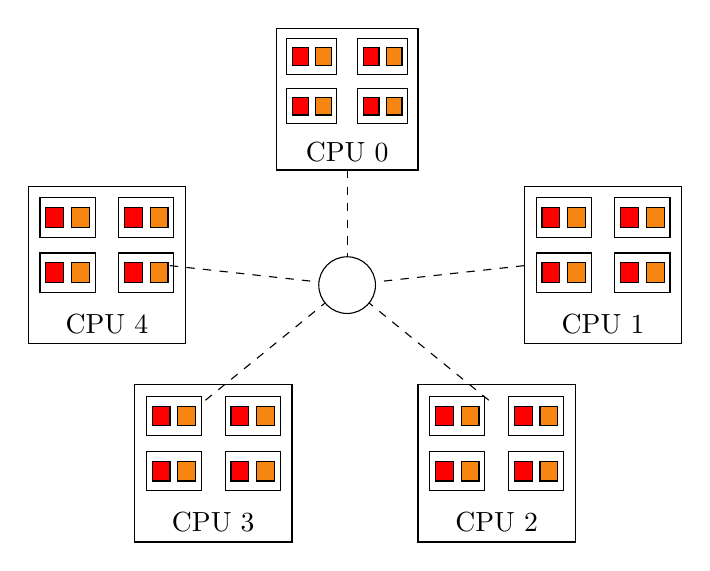
\begin{tikzpicture}[scale=0.9]

% CPUs
\begin{scope}[shift={(0, 0.25)}]
    \draw (0, 0) rectangle (2, 2);
    \node at (1, .25) {CPU 0};
    \draw (0.15, 1.35) rectangle (0.85, 1.85);
    \draw[fill=red] (0.225, 1.475) rectangle (0.45, 1.725);
    
    \visible<2->{
        \draw[fill=BurntOrange] (0.55, 1.475) rectangle (0.775, 1.725);
        
        \draw (1.15, 1.35) rectangle (1.85, 1.85);
        \draw[fill=red] (1.225, 1.475) rectangle (1.45, 1.725);
        \draw[fill=BurntOrange] (1.55, 1.475) rectangle (1.775, 1.725);
        
        \draw (0.15, 0.65) rectangle (0.85, 1.15);
        \draw[fill=red] (0.225, 0.775) rectangle (0.45, 1.025);
        \draw[fill=BurntOrange] (0.55, 0.775) rectangle (0.775, 1.025);
        
        \draw (1.15, 0.65) rectangle (1.85, 1.15);
        \draw[fill=red] (1.225, 0.775) rectangle (1.45, 1.025);
        \draw[fill=BurntOrange] (1.55, 0.775) rectangle (1.775, 1.025);
    };
\end{scope}
% \draw (0, 0.25) pic{cpu={0}};

\visible<3->{
    \draw (3.5, -2.2) pic{cpu={1}};
    \draw (2, -5) pic{cpu={2}};
    \draw (-2, -5) pic{cpu={3}};
    \draw (-3.5, -2.2) pic{cpu={4}};
    
    % Interconnects
    \draw[dashed] (-1.5, -1.1) -- (1.0, -1.625 + 0.25);
    \draw[dashed] (1.0, 0.25) -- (1.0, -1.625 + 0.25);
    \draw[dashed] (3.5, -1.1) -- (1.0, -1.625 + 0.25);
    \draw[dashed] (3, -3) -- (1.0, -1.625 + 0.25);
    \draw[dashed] (-1, -3) -- (1.0, -1.625 + 0.25);
    \draw[fill=white] (1.0, -1.625 + 0.25) circle (.4cm);
}
        \end{tikzpicture}
    \end{flushleft}
    \begin{tikzpicture}[overlay, shift={(10, 6)}]
        \visible<1->{
            \node[anchor=west, align=left, minimum size=2cm] at (0, 0) {Normal:\\\num{1} core};
        };
        \visible<2->{
            \node[anchor=west, align=left, minimum size=2cm] at (0.25, -1.6) {OpenMP:\\\num{4} cores (\num{8} HT)};
        };
        \visible<3->{
            \node<3->[anchor=west, align=left, minimum size=2cm] at (0.25, -3.3) {MPI + OpenMP:\\\num{20} cores (\num{40} HT)\\[-.25em]on \num{5} nodes};
        };
    \end{tikzpicture}
\end{frame}
%%%%%%%%%%%%%%%%%%%%%%%%%%%%%%%%%%%%%%%%%%%%%%%%%%%%%%%%%%%%%%%%%%%%

%%%%%%%%%%%%%%%%%%%%%%%%%%%%%%%%%%%%%%%%%%%%%%%%%%%%%%%%%%%%%%%%%%%%
\begin{frame}[fragile]{Parallelization Hints}
    \begin{itemize}
        \item It is allowed and highly advised \textbf{to hold the data redundant on each node}.
        \item Tree refinements on one level and the ones below are independent of each other.
        \item \textbf{Hint}: start with a sequential implementation, but keep the parallelization in mind (especially when choosing the used data structures).
        \item All data structures that need to be communicated via MPI must be serialized in some way.
        \item Pointers can not easily point into another MPI rank's memory.
        \item Pointer addresses change if you copy a structure.
        \item A structure with relative offsets can be more easily merged together than a structure with absolute offsets.
        \item Can the Barnes-Hut tree construction also be parallelized? 
    \end{itemize}
    \vfill
    \pause
    \DisplayRightArrow Think about \textbf{what} can be computed independently from each other! \\
    \DisplayRightArrow Think about \textbf{how} these computations can be parallelized! \\
    \DisplayRightArrow Think about \textbf{what} has to be communicated between different nodes!
\end{frame}
%%%%%%%%%%%%%%%%%%%%%%%%%%%%%%%%%%%%%%%%%%%%%%%%%%%%%%%%%%%%%%%%%%%%

\section{Visualization via ParaView}
%%%%%%%%%%%%%%%%%%%%%%%%%%%%%%%%%%%%%%%%%%%%%%%%%%%%%%%%%%%%%%%%%%%%
\begin{frame}[fragile]
  \frametitle{Visualization via ParaView}
  \begin{itemize}
      \item Visualizing the data via \link{https://www.paraview.org/}{ParaView}.
      \item Create one \texttt{.vtp} file, containing information about the current simulation state (e.g., body mass, position, energies of the system, $\dots$) for every visualization step on \textbf{every} MPI rank containing only the data it is responsible for.
      \item Create one \texttt{.pvd} file for the whole simulation on \textbf{one} MPI rank, referencing all \texttt{.vtp} files including the respective time step.
  \end{itemize}
\end{frame}
%%%%%%%%%%%%%%%%%%%%%%%%%%%%%%%%%%%%%%%%%%%%%%%%%%%%%%%%%%%%%%%%%%%%

\subsection{.pvd and .vtp Files}
%%%%%%%%%%%%%%%%%%%%%%%%%%%%%%%%%%%%%%%%%%%%%%%%%%%%%%%%%%%%%%%%%%%%
\begin{frame}[fragile]
  \frametitle{Example of a \texttt{.vtp} File with Two Bodies - 1}
  \setfontsize{5.3pt}
    \begin{minted}[bgcolor=lightgray!30,obeytabs=true,tabsize=2]{xml}
<?xml version="1.0"?>
<VTKFile type="PolyData" version="0.1" byte_order="LittleEndian" header_type="UInt64">
	<PolyData>
		<Piece NumberOfPoints="2" NumberOfVerts="2">
			<Points>
				<DataArray type="Float64" Name="position" NumberOfComponents="3" format="ascii">
                    0 0 0
                    -0.140728 -0.443901 -0.0233456
				</DataArray>
			</Points>
			<PointData>
        <DataArray type="Int32" Name="body_id" NumberOfComponents="1" format="ascii">
                    0
                    1
        </DataArray>
				<DataArray type="Float64" Name="velocity" NumberOfComponents="3" format="ascii">
                    5.37193e-06 -7.4078e-06 -9.4222e-08
                    0.0211745 -0.00710548 -0.00252296
				</DataArray>
				<DataArray type="Float64" Name="acceleration" NumberOfComponents="1" format="ascii">
                    9.15107e-06
                    0.022477
				</DataArray>
				<DataArray type="Float64" Name="mass" NumberOfComponents="1" format="ascii">
                    1.98847e+30
                    3.30101e+23
				</DataArray>
				<DataArray type="String" Name="name" NumberOfComponents="1" format="ascii">
                    83 117 110 0
                    77 101 114 99 117 114 121 0
				</DataArray>
  \end{minted}
\end{frame}
%%%%%%%%%%%%%%%%%%%%%%%%%%%%%%%%%%%%%%%%%%%%%%%%%%%%%%%%%%%%%%%%%%%%

%%%%%%%%%%%%%%%%%%%%%%%%%%%%%%%%%%%%%%%%%%%%%%%%%%%%%%%%%%%%%%%%%%%%
\begin{frame}[fragile]
  \frametitle{Example of a \texttt{.vtp} File with Two Bodies - 2}
  \setfontsize{5.3pt}
    \begin{minted}[bgcolor=lightgray!30,obeytabs=true,tabsize=2]{xml}
				<DataArray type="Int32" Name="orbit_class" NumberOfComponents="1" format="ascii">
                    0
                    1
				</DataArray>
			</PointData>
			<Verts>
				<DataArray type="Int64" Name="offsets">
                    1 2 
				</DataArray>
				<DataArray type="Int64" Name="connectivity">
                    0 1 
				</DataArray>
			</Verts>
		</Piece>
		<FieldData>
			<DataArray type="Float64" Name="kinetic energy" NumberOfTuples="1" format="ascii">
                    7.18489e+22
			</DataArray>
			<DataArray type="Float64" Name="potential energy" NumberOfTuples="1" format="ascii">
                    -1.37988e+23
			</DataArray>
			<DataArray type="Float64" Name="total energy" NumberOfTuples="1" format="ascii">
                    -6.6139e+22
			</DataArray>
			<DataArray type="Float64" Name="virial equilibrium" NumberOfTuples="1" format="ascii">
                    1.04138
			</DataArray>
		</FieldData>
	</PolyData>
</VTKFile>
  \end{minted}
\end{frame}
%%%%%%%%%%%%%%%%%%%%%%%%%%%%%%%%%%%%%%%%%%%%%%%%%%%%%%%%%%%%%%%%%%%%

%%%%%%%%%%%%%%%%%%%%%%%%%%%%%%%%%%%%%%%%%%%%%%%%%%%%%%%%%%%%%%%%%%%%
\begin{frame}
    \frametitle{\texttt{.vtp} File General Remarks}
    \begin{itemize}
        \item The \texttt{body\_id} must be unique for each body \textbf{across all} MPI ranks.
        \item The \texttt{name} must be saved converting each character to its ASCII representation and adding a \texttt{NULL} terminator. \\[.25em]
        Example:\quad
        \begin{tabular}{|c|c|c|c|}
            \hline
            S & u & n & \\\hline
            83 & 117 & 110 & 0 \\\hline 
        \end{tabular}
        \item The orbit~class is an integer corresponding to one of the classes on the bonus material
        \hyperlink{orbit_classes}{slide \ref{orbit_classes}}.
        \itFollows{Devise a suitable mapping!}
        \item The \texttt{offsets} and \texttt{connectivity} must start at \texttt{1} and \texttt{0} respectively on \textbf{each} MPI rank.
    \end{itemize}
\end{frame}
%%%%%%%%%%%%%%%%%%%%%%%%%%%%%%%%%%%%%%%%%%%%%%%%%%%%%%%%%%%%%%%%%%%%

%%%%%%%%%%%%%%%%%%%%%%%%%%%%%%%%%%%%%%%%%%%%%%%%%%%%%%%%%%%%%%%%%%%%
\begin{frame}[fragile]
  \frametitle{Example of a \texttt{.pvd} File}
  \textbf{Note:} \mintinline{xml}{timestep} \textbf{does not} correspond to the current time step number but to the current simulation time (in earth days)!
  \vfill
  Example with a visualization step width $vs = \SI{5}{\day}$ using two MPI ranks:
  \setfontsize{7.2pt}
  \begin{minted}[bgcolor=lightgray!30,obeytabs=true,tabsize=2]{xml}
<?xml version="1.0"?>
<VTKFile type="Collection" version="0.1" byte_order="LittleEndian" compressor="vtkZLibDataCompressor">
	<Collection>
		<DataSet timestep="0.0" group="" part="0" file="time_series/0/sim.0.vtp"/>
		<DataSet timestep="0.0" group="" part="1" file="time_series/1/sim.0.vtp"/>
		<DataSet timestep="5.0" group="" part="0" file="time_series/0/sim.1.vtp"/>
		<DataSet timestep="5.0" group="" part="1" file="time_series/1/sim.1.vtp"/>
		<DataSet timestep="10.0" group="" part="0" file="time_series/0/sim.2.vtp"/>
		<DataSet timestep="10.0" group="" part="1" file="time_series/1/sim.2.vtp"/>
		<DataSet timestep="15.0" group="" part="0" file="time_series/0/sim.3.vtp"/>
		<DataSet timestep="15.0" group="" part="1" file="time_series/1/sim.3.vtp"/>
	</Collection>
</VTKFile>
  \end{minted}
\end{frame}
%%%%%%%%%%%%%%%%%%%%%%%%%%%%%%%%%%%%%%%%%%%%%%%%%%%%%%%%%%%%%%%%%%%%

\subsection{ParaView}
%%%%%%%%%%%%%%%%%%%%%%%%%%%%%%%%%%%%%%%%%%%%%%%%%%%%%%%%%%%%%%%%%%%%
\begin{frame}[fragile]
	\frametitle{ParaView Basics - 1}
	Most important ParaView views and options:
	\setlength{\leftmargini}{-0.4cm}
    \setlength{\leftmarginii}{-0.4cm}
    \begin{description}
      \item[View $\rightarrow$ Properties] used for general visualization properties
      \begin{itemize}
          \item Use \texttt{Points} as \textit{Representation}.
          \item Use an appropriate \textit{Point Size}.
      \end{itemize}
      \item[View $\rightarrow$ Find Data] used to extract data satisfying a specific property
      \begin{itemize}
          \item Can be used to create different groups for, e.g., different orbit classes (these groups can then be visualized with different colors or \textit{Point Sizes}!).
          \item Use \texttt{name} in the \textit{Point Labels} drop-down menu to print the body name during the simulation.
          \item Can also be used to search for a specific body (\textbf{Note:} unfortunately it is not possible to search by the body name in ParaView!).
      \end{itemize}
      \item[View $\rightarrow$ Animation View] used for more control over the simulation visualization
      \begin{itemize}
          \item Select a previously generated (via \enquote{Find Data}) extraction.
          \item Select \texttt{Camera} and \texttt{Follow Data} in the two drop-downs and click the \textit{+}.
          \item ParaView now follows the specified data during the simulation!
      \end{itemize}
    \end{description}
\end{frame}
%%%%%%%%%%%%%%%%%%%%%%%%%%%%%%%%%%%%%%%%%%%%%%%%%%%%%%%%%%%%%%%%%%%%

%%%%%%%%%%%%%%%%%%%%%%%%%%%%%%%%%%%%%%%%%%%%%%%%%%%%%%%%%%%%%%%%%%%%
\begin{frame}[fragile]
	\frametitle{ParaView Basics - 2}
	\setlength{\leftmargini}{-0.4cm}
    \setlength{\leftmarginii}{-0.4cm}
    \begin{description}
      \item[Automate ParaView Tasks] \hfill\\
        \begin{itemize}
            \item Start recording via \textit{Tools $\rightarrow$ Start Trace}.
            \item Do all the stuff you want to be automated.
            \item Stop recording via \textit{Tools $\rightarrow$ Stop Trace}.
            \item A new window opens where you can further customize the macro.
            \item Save the script as macro via \textit{File $\rightarrow$ Save As Macro$\dots$}.
            \item The new macro can now be found under \textit{Macros}.
        \end{itemize}
      \item[Filters $\rightarrow$ Data Analysis $\rightarrow$ Plot Global Variables Over Time] \hfill\\\hspace{-.5cm}
        used to display the energy plot
      \item[File $\rightarrow$ Save Screenshot...] \hfill\\\hspace{-.5cm}
        used to save the \textbf{current} time step as an image
      \item[File $\rightarrow$ Save Animation...] \hfill\\\hspace{-.5cm}
        used the save the \textbf{whole} simulation as a video
    \end{description}
\end{frame}
%%%%%%%%%%%%%%%%%%%%%%%%%%%%%%%%%%%%%%%%%%%%%%%%%%%%%%%%%%%%%%%%%%%%
\section{Simulation}
%%%%%%%%%%%%%%%%%%%%%%%%%%%%%%%%%%%%%%%%%%%%%%%%%%%%%%%%%%%%%%%%%%%%
\begin{frame}[fragile]
  \frametitle{Running the Simulation}

The simulation must be executable on the command line as follows, whereby the command line parameters may be given in an arbitrary order!
\begin{center}
    \setfontsize{9pt}
    \mintinline{text}{./simulate --file data.csv --dt 1h --t_end 1y --vs 1d --vs_dir sim_out --theta 1.05}
    \mintinline{text}{./simulate  --dt 1h --vs 1d --t_end 1y --theta 1.05 --file data.csv --vs_dir sim_out}
\end{center}

\begin{description}
  \item[\texttt{--file}] the used simulation data file
  \item[\texttt{--dt}] the time step width $\Delta t$
  \item[\texttt{--t\_end}] the end time of the simulation
  \item[\texttt{--vs}] the visualization step width
  \item[\texttt{--vs\_dir}] the top most output directory for all visualization files
  \item[\texttt{--theta}] the threshold in the Barnes-Hut algorithm
\end{description}
\vfill
The above invocation simulates \mintinline{text}{data.csv} for one earth year with a resolution of one hour visualizing each day and writing all visualization files to the folder \mintinline{text}{sim_out/}.
\end{frame}
%%%%%%%%%%%%%%%%%%%%%%%%%%%%%%%%%%%%%%%%%%%%%%%%%%%%%%%%%%%%%%%%%%%%

%%%%%%%%%%%%%%%%%%%%%%%%%%%%%%%%%%%%%%%%%%%%%%%%%%%%%%%%%%%%%%%%%%%%
\begin{frame}[fragile]
  \frametitle{Running the Simulation - Time Duration Parameters}

    For a more intuitive command line experience, the values of the three command line parameters \texttt{--dt}, \texttt{--t\_end}, and \texttt{--vs} are positive, decimal numbers followed by one of \texttt{h} (hours), \texttt{d} (days), \texttt{m} (months), or \texttt{y} (years).
    \vfill
    Examples for valid values are: \SI{1}{\hour}, \SI{12}{\day}, \SI{3.5}{\month}, or \SI{1.25}{\year}. \\[.4em]
    Examples for invalid values are: \SI{-2}{\hour}, \SI{60}{\second}, or \num{1.5}\,\texttt{hd}.
    \vfill
    \pause
    \textbf{Note:} you should convert all values into earth days for your internal calculations:
    \begin{itemize}
        \item $\SI{1}{\hour} \equiv \SI{0.0416667}{\day}$
        \item $\SI{1}{\month} \equiv \SI{30.4167}{\day}$
        \item $\SI{1}{\year} \equiv \SI{365.25}{\day}$
    \end{itemize}
\end{frame}
%%%%%%%%%%%%%%%%%%%%%%%%%%%%%%%%%%%%%%%%%%%%%%%%%%%%%%%%%%%%%%%%%%%%

\subsection{Validation}
%%%%%%%%%%%%%%%%%%%%%%%%%%%%%%%%%%%%%%%%%%%%%%%%%%%%%%%%%%%%%%%%%%%%
\begin{frame}[fragile]
  \frametitle{Validation Hints for the Simulation}
  \begin{itemize}
    \item Use the ParaView visualization to validate your simulation:
    \begin{itemize}
        \item Is the simulation stable, i.e., do all planets and their moons have stable orbits?
        \item Use the known orbital periods of objects:
        \begin{itemize}
            \item Earth approx. \SI{1}{\year} (\SI{365.25}{\day})
            \item Mars approx. \SI{687}{\day}
            \item Jupiter approx. \SI{12}{\year} (\SI{4383}{\day}) 
            \item Europa (moon) approx. \SI{85}{\hour} (\SI{3.54}{\day})
        \end{itemize}
    \end{itemize}
    \item Use the Virial Equilibrium and the laws of mass and energy conservation as additional mechanisms to detect errors.
  \end{itemize}
  \vfill
  \pause
  \textbf{Attention!:}\\
  It may happen that Pluto and its moons will not form a stable system, i.e., some moons (mainly Kerberos and Hydra) will be ejected from the system. This is most likely \textbf{not} a bug in your simulation, but the consequence of insufficient data from JPL's Horizons website.\\[-.5em]
  \begin{spacing}{0.8}
      \setfontsize{8pt}
      For more information see: \\
      \texttt{S. Kenyon, B. Bromley: A Pluto-Charon Sonata IV. Improved Constraints on the Dynamical Behavior and Masses of the Small Satellites\textquotedblright (2022) (\url{https://arxiv.org/pdf/2204.04226.pdf})}
    \end{spacing}
\end{frame}
%%%%%%%%%%%%%%%%%%%%%%%%%%%%%%%%%%%%%%%%%%%%%%%%%%%%%%%%%%%%%%%%%%%%
\section{Important Deadlines}
%%%%%%%%%%%%%%%%%%%%%%%%%%%%%%%%%%%%%%%%%%%%%%%%%%%%%%%%%%%%%%%%%%%%
\againframe{important_deadlines}
%%%%%%%%%%%%%%%%%%%%%%%%%%%%%%%%%%%%%%%%%%%%%%%%%%%%%%%%%%%%%%%%%%%%


\end{document}
